\documentclass[graybox]{svmult}
%\documentclass{Springer_template_contributed_works/svmult}
%\usepackage{newtxmat}

\usepackage{acronym}
\usepackage{amsmath,amssymb}
\usepackage[aboveskip=1pt,labelfont=bf,labelsep=period,justification=raggedright,singlelinecheck=off]{caption}
\usepackage{changepage}
\usepackage{cite}
\usepackage{nameref,hyperref}
\usepackage[right]{lineno}
\usepackage[nopatch=eqnum]{microtype}

\usepackage{xcolor}
\usepackage{multirow}
\usepackage{ctable} % for \specialrule command
\usepackage{multirow} % to combine cells vertically in a table
\usepackage{graphicx}
\usepackage{subcaption}


% ############ From Springer Template ###############
\usepackage{type1cm}        % activate if the above 3 fonts are
                            % not available on your system
%
\usepackage{makeidx}         % allows index generation
\usepackage{graphicx}        % standard LaTeX graphics tool
                             % when including figure files
\usepackage{multicol}        % used for the two-column index
\usepackage[bottom]{footmisc}% places footnotes at page bottom


\usepackage{newtxtext}
\usepackage[varvw]{newtxmath}       % selects Times Roman as basic font
% ###################################################


\captionsetup[subfigure]{justification=centering}

\usepackage[outputdir=.]{minted}
\setminted{autogobble=true,linenos=true,frame=single,framerule=1pt,numbersep=-1.5em}

\bibliographystyle{abbrv}

% Header and Footer with logo
\usepackage{lastpage,fancyhdr,graphicx}
\usepackage{epstopdf}
\pagestyle{fancy}
\fancyhf{}
\rfoot{\thepage/\pageref{LastPage}}
\renewcommand{\headrulewidth}{0pt}
\renewcommand{\footrule}{\hrule height 2pt \vspace{2mm}}
\lfoot{\today}

\newcommand{\etal}{{\textit{et al. }}}
\newcommand{\mbx}{\mathbf{x}}
\newcommand{\mbu}{\mathbf{u}}
\newcommand{\mbp}{\mathbf{p}}
\newcommand{\mby}{\mathbf{y}}
\newcommand{\mbd}{\mathbf{d}}
\newcommand{\mbg}{\mathbf{g}}
\newcommand{\mbf}{\mathbf{f}}
\newcommand{\cmt}[1]{\textcolor{red} {[#1]}}
\providecommand{\keywords}[1]{\textbf{Keywords } #1}

% Create a new environment for code samples.
\newfloat{code}{tbp}{lop}
\floatname{code}{Code Sample}

% Create acronyms to use in text
\newacro{ode}[ODE]{Ordinary Differential Equation}
\newacro{oed}[OED]{optimal experimental design}
\newacro{fim}[FIM]{Fisher Information Matrix}

\begin{document}
% ########################################################################
% ########################################################################

\title*{Experimental design for predictive models in microbiology depending on environmental variables}

\author{
    Polina Gaindrik, Jonas Pleyer, Daniel Heger and Christian Fleck
}
\institute{
    Polina Gaindrik, Jonas Pleyer, Christian Fleck \at
    \href{https://www.fdm.uni-freiburg.de/spatsysbio}{University of Freiburg, Freiburg Center for Data Analysis and Modeling},
    Ernst-Zermelo-Str. 1, 79104 Freiburg, Germany
    \and
    Daniel Heger \at
    \href{https://tsenso.com/en/}{tsenso GmbH, Johannesstr. 19, 70176 Stuttgart, Germany}
}


\maketitle

% ########################################################################
% ########################################################################
\abstract{
%
The aim of predictive microbiology is the provision of tools and methods for predicting the growth, survival, and death of microorganisms in different food matrices under a range of environmental conditions. The parametrized mathematical models need to be calibrated using dedicated experimental data.
In order to efficiently plan experiments model-based experimental design is used. In this chapter, we explain model-based experimental design and provide step-by-step instructions for finding the optimal design using the well-known Baranyi\&Roberts growth model as an example. We provide the Python software {\it eDPM} for \ac{ode} -based models, such that the reader can apply model-based experimental design in his/her research context.
}
\keywords{Optimal experimental design, Parameter estimation, \ac{fim}, Identifiability, Uncertainty}
%
%
%
% ########################################################################
% ########################################################################
\section*{Introduction}
% \begin{figure}[h]
% 	\inputminted[linenos,firstline=57,lastline=79]{python}{../model-design-fischer-information-matrix/pool_model.py}
% 	\caption{Sample code written in Python~\cite{rossumPythonLanguageReference2010}.}
% \end{figure}
%
Mathematical modeling is widely used to describe, understand and predict the behavior of living systems.
In particular, in the field of Predictive Biology, one can find a large variety of works that dwell on building models of different levels of complexity controlled by model parameters, e.g., to describe bacterial growth \cite{bernaertsConceptsToolsPredictive2004}.
Predictive microbiology is a subfield of food microbiology that uses mathematical models to predict the behavior of microorganisms in food.
It is based on the premise that the behavior of microorganisms can be mathematically described by the use of mathematical models, which can take into account the effects of various factors such as temperature, pH, water activity, and the presence of preservatives, on the growth and survival of microorganisms.
These models can then be used to predict the behavior of microorganisms under different conditions, and to evaluate the effectiveness of various control measures, such as refrigeration, heat treatment, or the addition of preservatives.
Predictive microbiology has many applications in food safety, as it can be used to assess the risk of food-borne illness, to design safe food processing and storage practices, and to develop new food products with extended shelf-life.
For successful predictions it is essential that the model parameters can be estimated from experimental data.
Due to measurement noise, the parameters can only be estimated with some uncertainties.
That gives rise to a set of important questions: Can all parameters of the given model structure be estimated?
What should be measured and when? What are the confidence intervals for the parameters? How can the experimental effort be minimized?
Answering these questions equates to finding the \ac{oed}.
This results in optimized experimental conditions and/or measurement times which allows for a reduction of the experimental load without loss of information \cite{derlindenImpactExperimentDesign2013, balsa-cantoe.bangaj.r.COMPUTINGOPTIMALDYNAMIC2008}.
In general, the Experimental Design procedure can be used not only for the parameter estimation but also for model discrimination \cite{kreutzSystemsBiology2009, stamatiOptimalExperimentalDesign2016}.
However, in this chapter, we focus on Experimental Design for parameter estimation.
Comprehensive reviews can be found here: \cite{atkinsonDevelopmentsDesignExperiments1982, franceschiniModelbasedDesignExperiments2008,sunParameterEstimation2011,vilasPredictiveFood2016}.\\\linebreak
The whole parameter estimation process starts with choosing a model structure and defining observable quantities which the researcher is interested in.
Once this is chosen a first parameter set is selected based on literature review or prior data.
In order to fine-tune the experimental design setup to the given use-case, we need to choose an objective function that will be optimized.
Depending on the goal, a researcher faces an important choice; which of the several sometimes contradicting objectives should be chosen for a particular case?
For example, is it more desirable to have precise knowledge in a chosen set of parameters and less information about the remaining ones?
What is the best balance between experimental effort and precision?
Using multi-objective approaches, some attempts were made to answer these questions and to improve the experimental design by combining several objectives~\cite{telenOptimalExperimentDesign2012, logistRobustMultiobjectiveOptimal2011}.
For models which depend on external cues like temperature, it is {\it a priori} not clear whether constant variable conditions are more efficient for the parameter estimation \cite{versyckIntroducingOptimal1999,garciaQualityShelflifePrediction2015}.
Using the initial guess of parameters a first \ac{oed} is determined taking into account specific constraints, such as maximum number of measurements, measurement times, etc.
Next, the designed experiments need to be performed and this data results into a new estimation of the parameters.
If the confidence intervals of the parameters are sufficiently small, the scheme ends, otherwise one uses the new estimates as the starting point for the next experimental design (see Figure~\ref{fig:expdesign_scheme}).
The process can be repeated several times to increase the precision of the parameter estimates until the desired accuracy is achieved.
To test the scheme one can also perform numerical experiments and obtain {\it in-silico} data.
\begin{figure}[H]
    \centering
    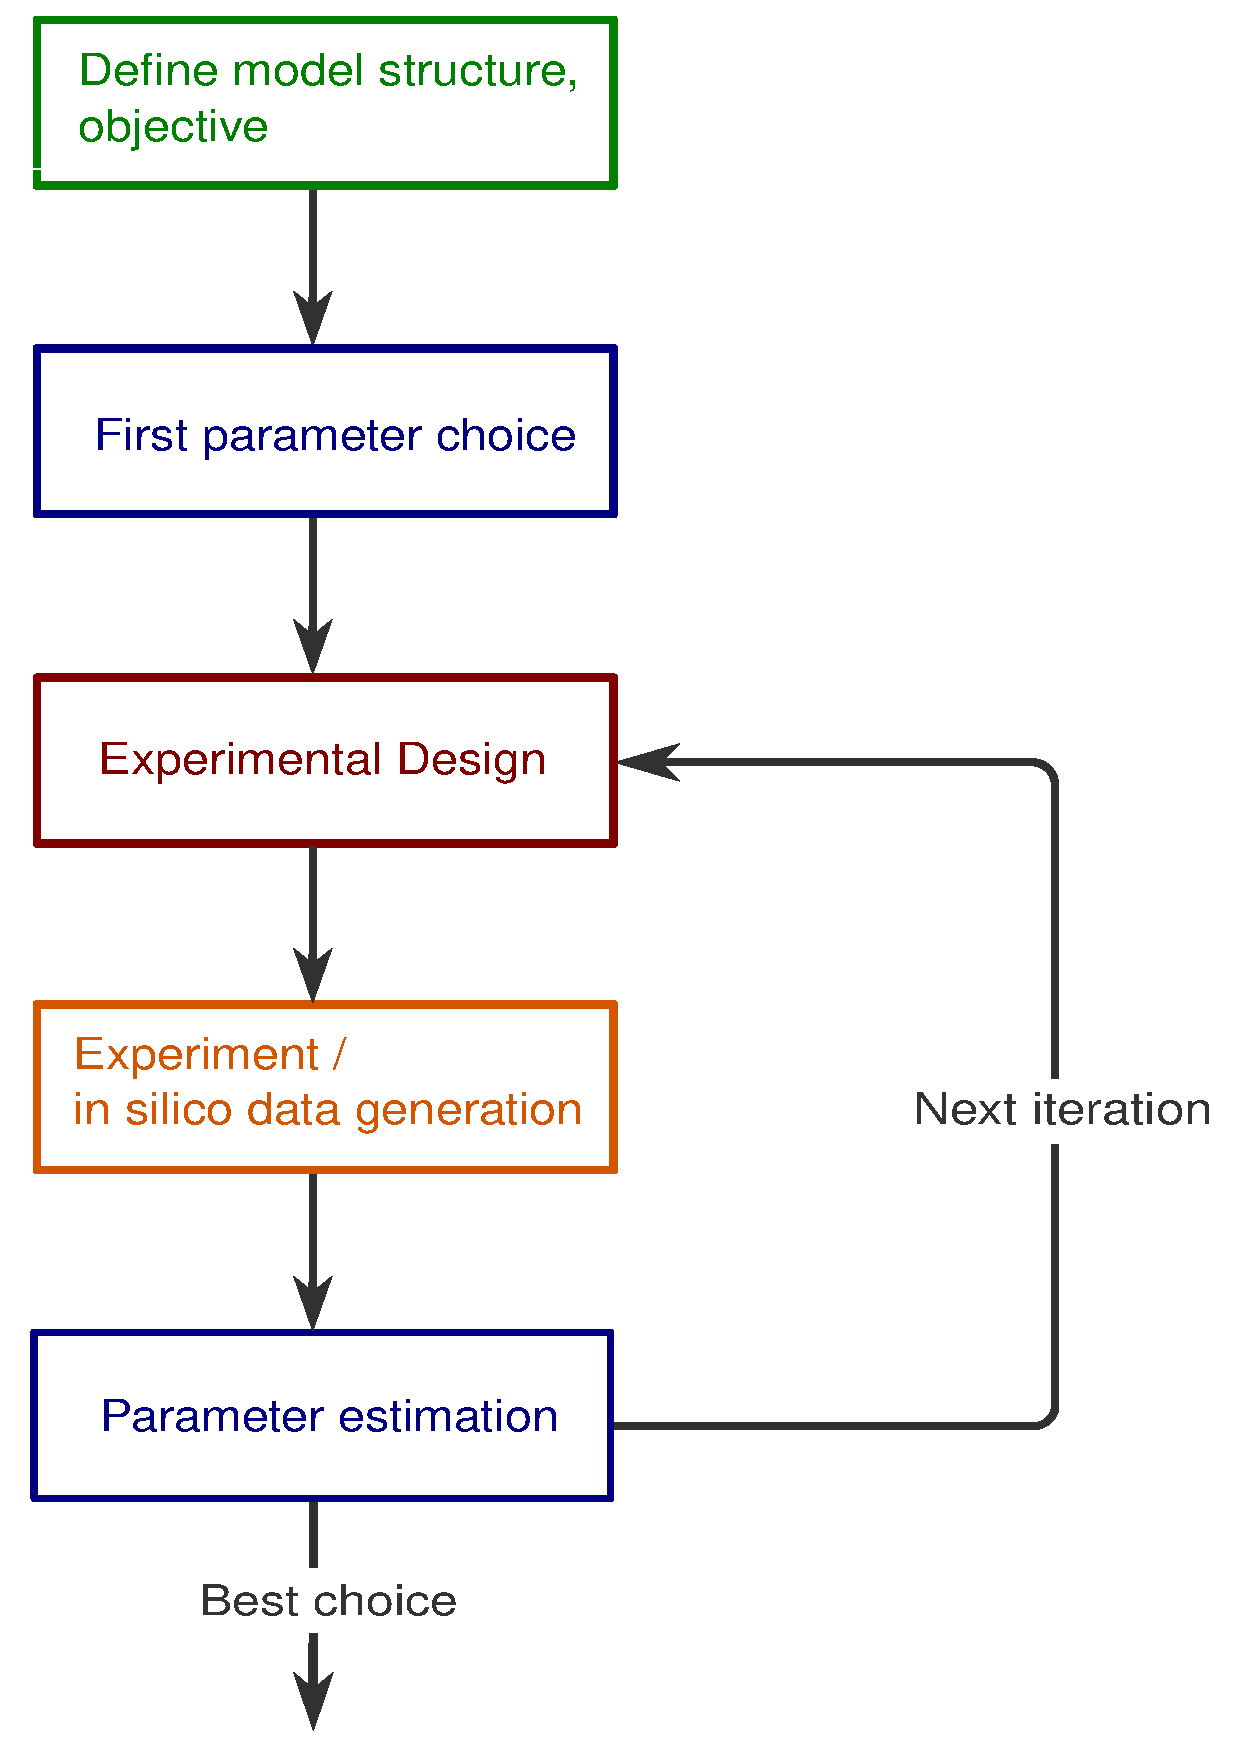
\includegraphics[scale=0.3]{Figures/scheme.pdf}
    \caption{{\footnotesize The workflow of the iterative process for model-based experimental design for parameter estimation.}}
    \label{fig:expdesign_scheme}
\end{figure}
%
%
%
% ########################################################################
% ########################################################################
\section*{Materials and Methods}
There are several software packages available for model-based experimental design~\cite{balsa-canto_amigo2_2016, zhang_optimal_2018, busetto_near-optimal_2013}.
These packages comprise a large number of tools and consequently require some time to understand how to use them.
We developed {\it eDPM} (Experimental Design for Predictive Microbiology), which focusses on ease of use.
It is a set of tools to calculate the Sensitivity and Fischer Information Matrix and do parameter space exploration in order to find optimal results.
We require a working installation of the popular scripting language Python $\geq3.7$~\cite{rossumPythonLanguageReference2010}.
For installation instructions, please refer to the website \href{https://www.python.org/downloads/}{python.org}.
In addition, we expect users to be able to write, execute and display output of scripts.
This tutorial can also be followed using jupyter notebooks \cite{jupyterteamJupyterNotebook}.
% TODO
Users can obtain it by installing {\it eDPM} from \href{https://pypi.org/project/edpm/0.0.1/}{pypi.org}.
The python website has guides for installing packages \href{https://packaging.python.org/en/latest/tutorials/installing-packages/}{packaging.python.org/}.
Most Unix-Based systems (e.g. GNU/Linux) and Mac-OS can use \mintinline[bgcolor=white,style=emacs]{bash}{pip}
\begin{minted}[bgcolor=white, linenos=false]{bash}
pip install eDPM
\end{minted}
or \mintinline[bgcolor=white,style=emacs]{bash}{conda} to install the desired package.
\begin{minted}[bgcolor=white, linenos=false]{bash}
conda install eDPM
\end{minted}
The \href{https://spatial-systems-biology-freiburg.github.io/eDPM/}{documentation} of the package is continuously updated.
After the installation of the package is complete, we open a file with a text editor of choice and simply start writing code.
We begin by writing a so-called she-bang which is responsible to signalize that this file is to be executed with python.
Afterwards, we import the needed packages.
\begin{code}[h]
    \begin{minted}[firstnumber=1]{python}
    #!/usr/bin/env python3

    import numpy as np
    from eDPM import *
    \end{minted}
    \caption{Import statements to use {\it eDPM}}
    \label{code:import_statements}
    % TODO make this FisInMa into a link
\end{code}
This will serve as the starting point for our script.\\
In the following, we will append more code to it and utilize the methods developed in {\it eDPM}~\cite{edpm2023}.
% TODO add citation which points to github repository
If line numbers are missing, these should be filled by blank lines for better readability.
%
%
% ########################################################################
\subsection*{Model Formulation}
\subsubsection*{Theory}
As a starting point it is necessary to define the mathematical model.
We restrict our discussion to biological system which can be described by a system of \aclp{ode}:
\begin{equation}
    \begin{cases}
    \dot \mbx (t) = \mbf(t, \mbx, \mbu, \mbp) \\
    \mbx (t_0) = \mbx_0.
    \label{eq:ode_general}
    \end{cases}
\end{equation}
Here $\mbx = (x_1, x_2, ..., x_n)$ is a vector of state variables of the system with initial condition $\mbx_0$, $t$ is the time, $\mbu$ is a vector of a externally controlled inputs into the system (e.g., supply of glucose or the external temperature) and $\mbp$ are the parameters of the system.
We assume that a subset of the parameters $\mbp$ is unknown and should be estimated from data.
Predominantly, the state variables cannot be directly observed, but rather the observables are functions of the state variables:
\begin{equation}
    \mby (t) = \mbg(t, \mbx (t), \mbu, \mbp) + \epsilon (t),
    \label{eq:observ_general}
\end{equation}
where the function $g$ is the observation or output function, and $\epsilon$ is the measurement noise.
The observational noise is often assumed to be an independently distributed Gaussian noise with zero mean and variance $\sigma^2$: $\epsilon (t) \sim N(0, \sigma^2)$, $\forall t$.\\
%
In this tutorial, we demonstrate the usage of Experimental Design on the widely employed mathematical model developed by Baranyi and Roberts \cite{baranyiDynamicApproach1994}, which was devised to describe bacterial growth.
The model introduces two state variables $\mbx = (x_1, x_2)$, where $x_1(t)$ denotes the cell concentration of a bacterial population at the time $t$
and $x_2(t)$ is the quantity defining the proportion of the growth rate specified by the environment, e.g., a limiting nutrient critical for bacterial growth.
\begin{equation}
    \begin{cases}
        \dot x_1(t) = f_1(x_1, x_2) = \frac{x_2(t)}{x_2(t) + 1} \mu^\text{max} \big(1 - \frac{x_1(t)}{x_1^\text{max}}\big) x_1(t)\\
        \dot x_2(t) = f_2(x_1, x_2) = \mu^\text{max}  x_2(t)
    \end{cases}.
    \label{eq:ode_BaranyiRoberts}
\end{equation}
Here $\mu^\text{max}$ determines the maximum growth rate, and $x_1^\text{max}$ is the maximal bacteria concentration due to environmental constraints.
The condition $x_2(0)$ allows to quantify the initial physiological state of the cells and, hence, the process of adjustment (lag-phase)~\cite{grijspeerdt_estimating_1999}.
To account for the influence of the temperature on the activity of the model, we will use the 'square root' or Ratkowsky-type model for the maximum growth rate~\cite{ratkowsky_relationship_1982}
\begin{equation}
    \sqrt{\mu^\text{max}} = b (T - T_\text{min}),
    \label{eq:RatkowskyModel}
\end{equation}
where $b$ is the regression coefficient, and $T_\text{min}$ is the minimum temperature at which the growth can occur.
As the observable we choose the bacteria count, i.e:
\begin{equation}
    y(t) = x_1(t)+\epsilon(t),
    \label{eq:observable}
 \end{equation}
a common choice in predictive microbiology.\\
The equations (\ref{eq:ode_BaranyiRoberts} - \ref{eq:observable}) fully define the system.
Here $x_1^\text{max}, b, T_\text{min}$ are the parameters that we estimate using observational data $y$ at measurement times $t_i$, and temperature $T$ is an input of the system.
Based on this model, we would like to optimize the choice of measurement times as well as temperatures (inputs) of the system to find the \acl{oed}.
%
% ########################################################################
\subsubsection*{Code}
In order to be able to solve the equations numerically, we first need first to define the \ac{ode} system in python.
As was explained in the previous sections, this system consists of the equation1 (\ref{eq:ode_general}) with initial values $t_0, \mbx_0$.
Next, we need to define all numerical values present in the system.
We distinguish between time points $t_i$ at which the result of the \ac{ode} is evaluated, inputs $\mbu$, which alter the behavior of our system (for example temperature, humidity, etc.), parameters $\mbp$, which are the quantities that we want to estimate and other arguments which might be needed to solve the \ac{ode}.
Table \ref{tab:fsm-variables} provides an overview of these quantities and gives corresponding names in the code.
In the following, we will step-by-step explain how to specify all variables needed by using the example of the Baranyi-Roberts Model (Eq. \ref{eq:ode_BaranyiRoberts}).
\begin{table}[H]
    \centering
    \begin{tabular}{ccccc}
        \specialrule{.1em}{.01em}{.05em}
        Description & Formula & Code \\[1ex]
        \toprule \vspace{1mm}
        \multirow{3}{*}{ODE} & $\mbf$                       & \mintinline[bgcolor=white,style=emacs]{python}{def ode_fun(t, x, u, p, ode_args)} \\
            & $\partial \mbf / \partial \mbx$ & \mintinline[bgcolor=white,style=emacs]{python}{def ode_dfdx(t, x, u, p, ode_args)} \\[0.5ex]
            & $\partial \mbf / \partial \mbp$ & \mintinline[bgcolor=white,style=emacs]{python}{def ode_dfdp(t, x, u, p, ode_args)} \\[0.5ex]
        \midrule
        \multirow{3}{*}{\shortstack{Observable\\(optional)}} & $\mbg$                       &  \mintinline[bgcolor=white,style=emacs]{python}{def obs_fun(t, x, u, p, ode_args)}\\[0.5ex]
         & $\partial \mbg / \partial x$ &  \mintinline[bgcolor=white,style=emacs]{python}{def obs_dgdx(t, x, u, p, ode_args)}\\[0.5ex]
                        & $\partial \mbg / \partial p$ &  \mintinline[bgcolor=white,style=emacs]{python}{def obs_dgdp(t, x, u, p, ode_args)}\\[0.5ex]
        \midrule
        Initial value   & $\mbx_0$ & \mintinline[bgcolor=white,style=emacs]{python}{x0}\\[0.5ex]
        Initial time    & $t_0$ & \mintinline[bgcolor=white,style=emacs]{python}{t0}\\[0.5ex]
        Time points     & $t_i$ & \mintinline[bgcolor=white,style=emacs]{python}{t}\\[0.5ex]
        Inputs          & $\mbu$   & \mintinline[bgcolor=white,style=emacs]{python}{u}\\[0.5ex]
        Parameters      & $\mbp$   & \mintinline[bgcolor=white,style=emacs]{python}{p}\\[0.5ex]
        Other arguments &       & \mintinline[bgcolor=white,style=emacs]{python}{ode_args}\\[0.5ex]
        \bottomrule
    \end{tabular}
    \caption{Summary of user-defined functions and variables.}
\label{tab:fsm-variables}
\end{table}
\paragraph{Defining the \acs{ode}}
We must define a few functions in python.
The first function will be the right-hand side of equation (\ref{eq:ode_general}), i.e., we need to implement the Baranyi-Roberts model (\ref{eq:ode_BaranyiRoberts}) into a function.
The implementation can be seen in Figure \ref{code:code_baranyi_roberts_ode_fun}.
We explain the individual steps to create this function in Code Sample~\ref{code:code_baranyi_roberts_ode_fun}.
\begin{code}[h]
    \begin{minted}[firstnumber=6]{python}
    # The function name can be chosen freely, but the order
    # of required function arguments is fixed by the definition.
    def baranyi_roberts_ode(t, x, u, p, ode_args):
        # Unpack the input vectors x,u,p for easy access
        # of their components
        (x1, x2) = x
        (Temp, ) = u
        (x_max, b, Temp_min) = p

        # Calculate the maximum growth rate
        mu_max = b**2 * (Temp - Temp_min)**2

        # Calculate the right hand side of the \ac{ode}, store
        # it in a list [ ... ] and return it.
        return [
            mu_max * (x2/(x2 + 1)) * (1 - x1/x_max) * x1,
            mu_max * x2
        ]
    \end{minted}
    \caption{
        Definition of the Baranyi-Roberts \ac{ode} model.
    }
    \label{code:code_baranyi_roberts_ode_fun}
\end{code}
%
% ########################################################################
\subsection*{Parameter Estimation}
After defining the model, the user needs to provide an initial parameter set.
This could be chosen from the literature or estimated from previously gathered experimental data.
It is common to assume that the observational or measurement noise is Gaussian white noise (e.g., no temporal correlations) with zero mean and variance $\sigma(t)^2$: $\epsilon(t) \sim N(0, \sigma(t)^2)$, $\forall t$.
In this case the logarithm of the likelihood function (log-likelihood) is given by~\cite{kreutzProfileLikelihood2013}:
\begin{equation}
    \ln L(\mbp) \propto - \sum_{i}\frac{ \big(\mathbf{g}^{i}(\mbp) - \mbd^{i}\big)^2}{2 \sigma_{i}^2}.
    \label{eq:likelihood_Gaussian}
\end{equation}
We introduced the following short hand notations:
\begin{itemize}
\item $\mbd^{i}$: data measured at time $t=t_i$
\item $\mathbf{g}^{i}(\mbp)$: the observation function depending on the parameter vector $\mbp$ evaluated at time $t=t_i$
\item $\sigma_{i}^2$: variance of the observational noise at time $t=t_i$.
\end{itemize}
The method of maximum likelihood consists in searching for the parameter vector $\mbp$ which maximizes the (log-)likelihood~\cite{gaborRobustEfficient2015}.
%
%
% ########################################################################
\subsection*{Experimental Design}
Following our definition of the model and setting the initial parameter vector $\mbp_0$ we can proceed to the Experimental Design.
In essence, Experimental Design comprises maximizing an objective function depending on the model, the initial parameter vector $\mbp_0$, external input $\mbu$ into the system, and a set of discrete observation times $t_i$ at which the potential measurements should be performed.
The objective function needs to quantify the information the observation $\mby$ has about the parameter vector $\mbp$.
A common choice here is constructing objective functions based on the \acf{fim} \cite{lyTutorialFisher2017}.
According to the so-called 'Cramer-Rao inequality', the Fisher information is inversely proportional to the minimal squared estimation error \cite{friedenExploratoryData2010}.
%Therefore, we choose some function of the FIM and optimize this objective function instead. 
%Due to this relationship, the \ac{fim} can be used as an estimate to 
%Due to this relationship maximization of the information leads to a minimization of the variance or uncertainty in the parameters.
This relation justifies using the FIM to improve our experimental design.
%Due to this relationship maximization of the information leads to an improvement of the experimental design.
In the following we explain one of the ways to calculate the \ac{fim} for an \acp{ode} system (\ref{eq:ode_general}) and the observable function (\ref{eq:observ_general}) \cite{lyTutorialFisher2017}.
%
%
% ########################################################################
\subsubsection*{Sensitivity Calculation}
An easy way to calculate the \ac{fim} uses local sensitivities of the observables $y$, that are in turn calculated from local sensitivities of the internal variables $x$~\cite{versyckIntroducingOptimal1999, banks_generalized_2010}.
Assume that functions $\mbf$ and $\mbg$ are differentiable functions with respect to the state variables $\mbx$ and parameters $\mbp$.
The local sensitivities of $\mbx$ are defined by $s^x_{ij} = (\mathrm{d} x_i / \mathrm{d} p_j )$.
These can be calculated using an enhanced system of the \acp{ode}:
\begin{equation}
    \begin{cases}
    \dot x_i (t) = f_i(t, \mbx, \mbu, \mbp)\\
    \dot s^x_{ij} = \sum_k \frac{\partial f_i}{\partial x_k} s^x_{kj} + \frac{\partial f_i}{\partial p_j}
    \end{cases}.
\label{eq:ode_and_sensitiv}
\end{equation}
For the \ac{fim} we need the sensitivities of observables functions $(\mathrm{d} y_i / \mathrm{d} p_j) = s_{ij}$.
We determine these at a certain times $t_m$ and input $u_n$ using the solutions of $s^x_{ij}$:
\begin{equation}
    s_{ij} (t_m, u_n) = \sum_k \frac{\partial g_i}{\partial x_k}\bigg|_{t_m, u_n} s_{kj}^x (t_m, u_n) + \frac{\partial g_i}{\partial p_j}\bigg|_{t_m, u_n}.
\label{eq:observ_sensitivities}
\end{equation}
\\
In the case the parameters are of very different scale (e.g., on the second and on the day scale), it may be advisable to use the relative or normalized sensitivities to improve not the absolute but the relative accuracy of the parameter estimates.:
\begin{equation}
    \tilde{s}_{ij} (t_m, u_n) =\frac{\mathrm{d}\ln(y_i)}{\mathrm{d}\ln(p_j)} = \frac{\mathrm{d} y_i}{\mathrm{d} p_j} \frac{p_j}{y_i}\bigg|_{t_m, u_n}.
\label{eq:relat_sensitivities}
\end{equation}
These sensitivities are the elements of the sensitivity matrix \cite{stigterObservabilityComplex2017}.
For example, in case of two observables $\mby = (y_1, y_2)$, two different inputs $\mbu = (u_1, u_2)$, $N$ different measurement times and $N_p$ parameters, sensitivity matrix reads:

\begin{equation}
    S =
\begin{pmatrix}
s_{11} (t_1, u_1) & ... & s_{1 N_p}(t_1, u_1) \\
\vdots  &   & \vdots  \\
s_{11} (t_{N}, u_1) & ... & s_{1 N_p} (t_{N}, u_1)\\
s_{11} (t_1, u_2) & ... & s_{1 N_p}(t_1, u_2) \\
\vdots  &   & \vdots  \\
s_{11} (t_N, u_2) & ... & s_{1 N_p} (t_N, u_2)\\

s_{21} (t_1, u_1) & ... & s_{2 N_p}(t_1, u_1) \\
\vdots  &   & \vdots  \\
s_{21} (t_{N}, u_1) & ... & s_{2 N_p} (t_{N}, u_1)\\
s_{21} (t_1, u_2) & ... & s_{2 N_p}(t_1, u_2) \\
\vdots  &   & \vdots  \\
s_{21} (t_N, u_2) & ... & s_{2 N_p} (t_N, u_2)
\end{pmatrix}
\label{eq:sens_matrix}
\end{equation}
This matrix will be used to directly calculate the \ac{fim}:
\begin{equation}
    F = S^T Q^{-1} S.
\end{equation}
Here, $Q$ is the covariance matrix of measurement error~\cite{cintron-arias_sensitivity_2009, balsa-cantoComputationalProcedures2008}.
If the measurements are independent, then only the diagonal elements of the matrix are non-zero:
\begin{equation}
    Q =
\begin{pmatrix}
    \sigma_{1}^2(t_1, u_1) & 0                      & 0                      & \dots  & 0                     \\
    0                      & \sigma_{1}^2(t_2, u_1) & 0                      & \dots  & 0                     \\
    0                      & 0                      & \sigma_{1}^2(t_1, u_2) & \dots  & 0                     \\
    \vdots                 & \vdots                 & \vdots                 & \ddots & \vdots                \\
    0                      & 0                      & 0                      & \dots  & \sigma_{2}^2(t_N, u_2)
\end{pmatrix},
\label{eq:covar_matrix}
\end{equation}
where $\sigma_{i}^2 (t_m, u_n)$ is the error of the measurements of observable $y_i$ at time point $t_m$ with input $u_n$.
The error can be either estimated from data or approximated by some error model.
For example, one may consider that the error contribution consists of an absolute part that stays constant and a relative part that is proportional to the observable values.
Then the diagonal elements of the covariance matrix take form:
\begin{equation}
\label{eq:error_model}
    \sigma_{i}^2 (t_m, u_n) = \gamma_\text{abs} + \gamma_\text{rel} \cdot y_i(t_m, u_n),
\end{equation}
where $\gamma_\text{abs}$ and $\gamma_\text{rel}$ are the coefficients determining the absolute and the relative error contribution, respectively.
In case one uses relative sensitivities $\tilde{s}_{ij} (t_m, u_n)$, one needs to use relative measurements errors for the matrix $Q$:
\begin{equation}
    \tilde{\sigma}_{i}^2 (t_m, u_n) = \frac{\sigma_{i}^2 (t_m, u_n)}{y^2_i(t_m, u_n)}.
\end{equation}
%
% ########################################################################
\subsubsection*{Numerical Sensitivity Calculation}
For the calculation of the sensitivities (Eq. \ref{eq:ode_and_sensitiv}) we need to supply the derivatives of $f$ with respect to the parameters and state variables.
We define $\mbx=(x_1,x_2,x_3)$ and $\mbp=(p_1,p_2,p_3)$ with $p_1=x_{max}$, $p_2=b$ and $p_3=T_\text{min}$.
Firstly, we calculate the mathematical derivatives $\partial f_i/\partial p_j$ and $\partial f_i/\partial x_j$ and then implement the corresponding functions.
The first component of the Baranyi-Roberts model reads:
\begin{equation}
\label{eq:rob_bar_model}
    \dot x_1(t) = f_1(t, \mbx, \mbu, \mbp) = \mu^\text{max} \frac{x_2(t)}{x_2(t) + 1} \left(1 - \frac{x_1(t)}{x_1^\text{max}}\right) x_1(t),
\end{equation}
where $\sqrt{\mu^\text{max}}=b(T-T_\text{min})$.
It follows:
\begin{alignat}{6}
    \frac{\partial\mu^\text{max}}{\partial p_1} &= 0\\
    \frac{\partial\mu^\text{max}}{\partial p_2} &= 2b(T-T_\text{min})^2 &=& &&\frac{2\mu^\text{max}}{b}\\
    \frac{\partial\mu^\text{max}}{\partial p_3} &= -2b^2(T-T_\text{min}) &=& &-&\frac{2\mu^\text{max}}{T-T_\text{min}}
\end{alignat}
and consequently:
\begin{alignat}{7}
    \frac{\partial f_1}{\partial p_1}(t) &= \mu^\text{max} &&\frac{x_2(t)}{x_2(t) + 1} &\frac{x_1(t)}{\left(x_1^\text{max}\right)^2} &&x_1(t)\\
    \frac{\partial f_1}{\partial p_2}(t) &= \frac{2\mu^\text{max}}{b} &&\frac{x_2(t)}{x_2(t) + 1} &\left(1 - \frac{x_1(t)}{x_1^\text{max}}\right) &&x_1(t)\\
    \frac{\partial f_1}{\partial p_3}(t) &= -\frac{2\mu^\text{max}}{T-T_\text{min}} &&\frac{x_2(t)}{x_2(t) + 1} &\left(1 - \frac{x_1(t)}{x_1^\text{max}}\right) &&x_1(t).
\end{alignat}
Similarly, the derivatives $\partial f/\partial x_i$ are given by:
\begin{alignat}{7}
    % TODO
    \frac{\partial f_1}{\partial x_1}(t) &= \mu^\text{max} &\frac{x_2(t)}{x_2(t) + 1} && \left(1-2\frac{x_1(t)}{x_1^\text{max}}\right) &&\\
    \frac{\partial f_1}{\partial x_2}(t) &= \mu^\text{max} &\frac{1}{(x_2(t)+1)^2} && \left(1 - \frac{x_1(t)}{x_1^\text{max}}\right) &&x_1(t).
    % TODO
\end{alignat}
The readers are encouraged to calculate the components $\partial f_2/\partial p_i$ and $\partial f_2/\partial x_i$ as an exercise.
The resulting implemented functions in python can be seen in Code Sample~\ref{code:code_baranyi_roberts_ode_fun_derivatives}.
\begin{code}[H]
    \begin{minted}[firstnumber=25]{python}
    def ode_dfdp(t, x, u, p, ode_args):
        (x1, x2) = x
        (Temp, ) = u
        (x_max, b, Temp_min) = p
        mu_max = b**2 * (Temp - Temp_min)**2
        return [
            [
                mu_max * (x2/(x2 + 1)) * (x1/x_max)**2,
                2 * b * (Temp - Temp_min)**2 * (x2/(x2 + 1))
                    * (1 - x1/x_max)*x1,
                -2 * b**2 * (Temp - Temp_min) * (x2/(x2 + 1))
                    * (1 - x1/x_max)*x1
            ],
            [
                0,
                2 * b * (Temp - Temp_min)**2 * x2,
                -2 * b**2 * (Temp - Temp_min) * x2
            ]
        ]

    def ode_dfdx(t, x, u, p, ode_args):
        (x1, x2) = x
        (Temp, ) = u
        (x_max, b, Temp_min) = p
        mu_max = b**2 * (Temp - Temp_min)**2
        return [
            [
                mu_max * (x2/(x2 + 1)) * (1 - 2*x1/x_max),
                mu_max * 1/(x2 + 1)**2 * (1 - x1/x_max)*x1
            ],
            [
                0,
                mu_max
            ]
        ]
    \end{minted}
    \caption{Derivatives of the function $f$ of the Baranyi-Roberts model \ac{ode}.}
    \label{code:code_baranyi_roberts_ode_fun_derivatives}
\end{code}
%
% ########################################################################
\subsubsection*{Define numerical values}
After the definition of the structure of the \ac{ode}, we need to specify numerical values.
It is good practice, to gather such definitions in the \mintinline[bgcolor=white,style=emacs]{python}{__main__} method of the python program as it was done in Code Sample~\ref{code:code_write_main_function_start}.
We start by defining the parameters of the \ac{ode} (line 64) and afterwards the initial values (line 67).
Next, we constrain the optimization routine to find the best possible time points in the interval $t_i\in\left[t_\text{low},t_\text{high}\right]$.
To do this, we write the times as a dictionary with entries \mintinline[bgcolor=white,style=emacs]{python}{{"lb":t_low, "ub":t_high, "n":n_times}} where \mintinline[bgcolor=white,style=emacs]{python}{"lb"} and \mintinline[bgcolor=white,style=emacs]{python}{"ub"} are the lower and the upper bound while \mintinline[bgcolor=white,style=emacs]{python}{n_times} describes the number of discrete time points at which we want to sample the system (line 70).
In contrast, if we wanted to specify explicit values for the sampling points, we would have needed to supply a list of time values or a \mintinline[bgcolor=white,style=emacs]{python}{np.ndarray} directly.
One can see this approach  in line 78 of the code example.
Here, we supply a \mintinline[bgcolor=white,style=emacs]{python}{np.ndarray} with explicit values, thus fixing the sampling points them for the optimization routine.
\begin{code}[h]
    \begin{minted}[firstnumber=62]{python}
    if __name__ == "__main__":
        # Define parameters
        p = (2e4, 0.02, -5.5)

        # Define initial conditions
        x0 = np.array([50, 1])

        # Define interval and number of sampling points for times
        times = {"lb":0.0, "ub":100.0, "n":4}

        # Define explicit temperature points
        Temp_low = 2.0
        Temp_high = 12.0
        n_Temp = 3

        # Summarize all input definitions in list (only temperatures)
        inputs = [
            np.linspace(Temp_low, Temp_high, n_Temp)
        ]
    \end{minted}
    \caption{
        The main function will encompass every step in our experimental design approach.
        In the beginning, we insert the actual values for our model definition.
    }
    \label{code:code_write_main_function_start}
\end{code}
\subsubsection*{Defining Explicit Values and Sampling}
There are two distinct ways to define inputs of the model.
First, one can fix (multiple) explicit values for an input variable.
The experiment will then be solved for only these values without optimizing them.
Secondly, one can also optimize inputs of the system.
The difference between choosing explicit values and specifying a sampling range may be subtle at first glance, but in turn allows to very easily switch between fixed values and optimized sampling points.
For example, suppose we want to optimize the temperature at which the experiments are performed, which means we let the optimization algorithm pick the optimal temperature points such that the information gathered from the system is maximized.
Then the difference between defining explicit values for the temperatures and defining an interval for optimization can be understood in code sample~\ref{code:difference_explicit_sampling}.\newline
\begin{code}[h]
    \begin{minted}[linenos=false]{python}
    # This will fix values explicitly
    inputs = [
        np.linspace(Temp_low, Temp_high, n_Temp)
    ]
    # >>> inputs
    # [array([2., 7., 12.])]


    # This will sample in the interval (Temp_low, Temp_high)
    # with n_Temp points.
    inputs = [
        {"lb":Temp_low, "ub":Temp_high, "n":n_Temp}
    ]
    # >>> inputs
    # [{'lb': 2.0, 'ub': 12.0, 'n': 3}]


    \end{minted}
    \caption{Difference between choosing explicit values and sampling over a given interval.}
    \label{code:difference_explicit_sampling}
\end{code}%
The different variables can be treated individually as needed.
Suppose, we have a system with temperatures and humidity as input variables.
We could decide to have the temperature optimized, but fix the humidity explicitly, because experimentally one can change the temperature continuously (or in discrete steps) but is restricted regarding the humidity.
In our code, we simply would mix explicit and sampled definitions for individual inputs (see code sample~\ref{code:mix_sampling_explicit}).
\begin{code}[h]
    \begin{minted}[linenos=false]{python}
        inputs = [
            # These values will be sampled
            {"lb":Temp_low, "ub":Temp_high, "n":n_Temp},
            # These are fixed
            np.array([0.4, 0.45, 0.5, 0.55])
        ]
    \end{minted}
    \caption{Mixing of explicit and sampling for inputs.}
    \label{code:mix_sampling_explicit}
\end{code}
%
% ########################################################################
\subsubsection*{Define Model}
After we have decided on the numerical values for our model, we need to put everything together.
The \mintinline[bgcolor=white,style=emacs]{python}{FisherModel} class serves as the entry point.
Here, we simply supply every previously made definition of variables and methods.
When using the syntax as shown in code sample~\ref{code:model_definition}, the order of arguments does not matter.
However, when only using \mintinline[bgcolor=white,style=emacs]{python}{FisherModel(x0, 0.0, ...)}, please pay attention to the order of arguments.
\begin{code}[H]
    \begin{minted}[autogobble=false,firstnumber=82]{python}
    # Create the FisherModel which serves as the entry point
    #  for the solving and optimization algorithms
    fsm = FisherModel(
        ode_x0=x0,
        ode_t0=0.0,
        ode_fun=baranyi_roberts_ode,
        ode_dfdx=ode_dfdx,
        ode_dfdp=ode_dfdp,
        times=times,
        inputs=inputs,
        parameters=p
    )
    \end{minted}
    \caption{Define the full model.}
    \label{code:model_definition}
\end{code}
\noindent For a full list of optional arguments, we refer to the \href{https://spatial-systems-biology-freiburg.github.io/eDPM/}{documentation} of the package.
%
% ########################################################################
%
% ########################################################################
\subsubsection*{Optimality Criteria}
In the next step we choose the objective function also called optimality criterion.
Optimization of the different objectives leads to different experimental design outcomes.
The most popular criteria are~\cite{balsa-cantoe.bangaj.r.COMPUTINGOPTIMALDYNAMIC2008, dette_designing_1997, walter_qualitative_1990}:
\begin{itemize}
\item \textbf{D-optimality criterion} maximizes the determinant $\det (F)$ of the \ac{fim}.
 Translated to the parameter space, it means that the volume of the confidence region (see Figure~\ref{fig:opt_criteria}) (or the geometric mean of all errors) is minimized.
 The size of the confidence region is determined by a confidence level, which is typically chosen $90 \%$ or $95 \%$.
 The confidence level can be interpreted as a probability value that the best
 parameter fit will belong to this area in case of repeating the experiment and estimations multiple times.
 The confidence region is usually presented as a confidence ellipsoid.
 D-optimality is the most widely used criterion and is suitable even in case of such parameter transformations as rescaling.
\item \textbf{E-optimality criterion} maximizes the smallest eigenvalue $\lambda_{\min}$ of the \ac{fim}, which is the same as reducing only the largest estimation error.
\item \textbf{A-optimality criterion} maximizes the sum of all eigenvalues $\sum_i \lambda_i$, which can be interpreted as minimizing the algebraic mean of all errors.
\item \textbf{Modified E-optimality criterion} maximizes the ratio between the minimal and maximal eigenvalue $\lambda_{\min} / \lambda_{\max}$ and reduces correlation between two parameters corresponding to these eigenvalues.

\end{itemize}
Each of the criteria has its pros and cons so the reader should have a closer look at the various properties of these criteria, for instance, in Franceschini's and Macchietto's paper \cite{franceschiniModelbasedDesignExperiments2008}.
For the geometrical interpretation of the criteria using the confidence region shown in Figure~\ref{fig:opt_criteria}.

\begin{figure}[H]
    \centering
    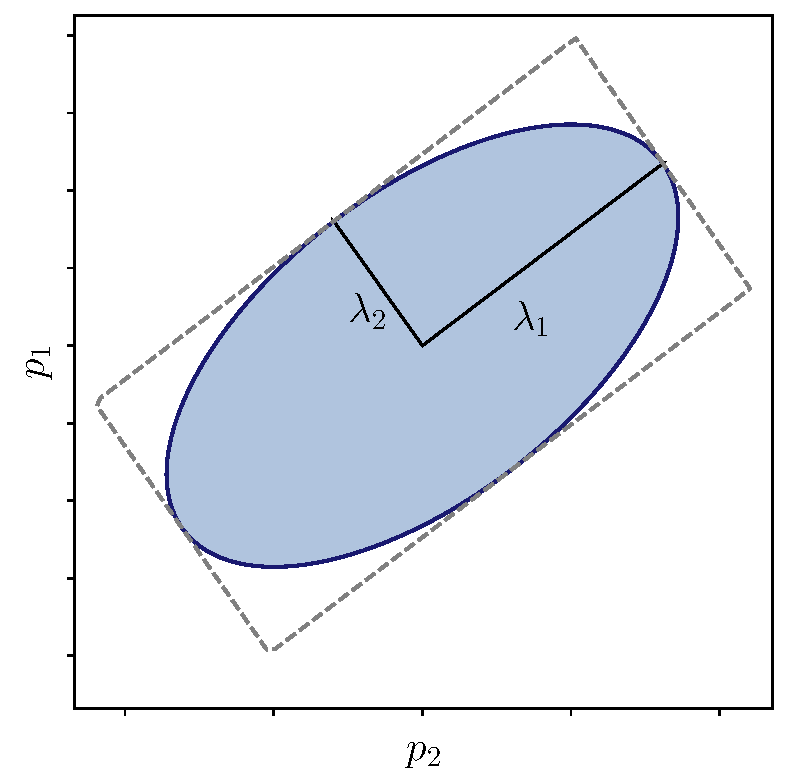
\includegraphics[scale=0.6]{Figures/optimality_criteria.pdf}
    \caption{{\footnotesize The confidence ellipsoid projection to the ($p_1$, $p_2$) parameter space.
    The ellipsoid shows the geometrical meaning of the optimality criteria.
    The center of the ellipsoid represents the estimated parameter values.
    The radii are the uncertainties of the estimates associated with different eigenvalues of the \ac{fim} $\lambda_1$, $\lambda_2$ ($\lambda_1 < \lambda_2$).
    The D-optimality aims to minimize the volume of the ellipsoid, the E-optimality minimizes the largest radius, A-optimality minimizes the perimeter of the rectangle that encloses the ellipse (dashed gray line), and, finally,  modified E-optimality tends to make the ellipse as spherical as possible.}}
    \label{fig:opt_criteria}
\end{figure}
%
% ########################################################################
\subsubsection*{Optimization}
After defining the objective function based on the \ac{fim} the next step is to optimize the chosen optimality criteria.
Finding the Experimental Design corresponds to finding the global maximum of the objective, which can be formulated as an optimal control problem~\cite{espie_optimal_1989}.
This problem has been widely studied, and multiple numerical solution algorithms for both local and global optimization were introduced~\cite{esposito_global_2000, bangaImprovingFoodProcessing2003, ali_numerical_1997, runarsson_stochastic_2000}.
In the supplied toolbox {\it eDPM}, three methods were implemented: Differential evolution, basin-hopping, and the so-called “brute force” method.
We give in the following a brief summary of the implemented methods.
For more information the reader should turn to the available literature, e.g.,~\cite{stornDifferentialEvolutionSimple1997, wales_global_1997}.
\newline
%
The differential evolution algorithm developed by Storn and Price (1996)~\cite{stornDifferentialEvolutionSimple1997} is one of the stochastic global optimization methods appropriate for nonlinear dynamic problems.
Such types of algorithms have mild computational load but one cannot be sure that the absolute optimum is reached~\cite{balsa-cantoe.bangaj.r.COMPUTINGOPTIMALDYNAMIC2008}.
For differential evolution an initial population of candidate vectors for the Experimental Design (sampling times and inputs) is randomly chosen from the region of available values.
Then each vector mutates by mixing with one of other candidate vectors.
To a chosen vector from the initial population $D_0$, we add a weighted difference between two other randomly chosen vectors from the same set $(D_\text{rand1} - D_\text{rand2})$.
This process is called mutation and a new vector $D_m$ is obtained.
The next step is to construct a new trial solution.
This is done by choosing the elements of the trial vector either from the initial $D_0$ or the mutated $D_m$ vectors.
For each new element of trial vector, a random number drawn uniformly from the interval [0, 1) and compared to the so-called recombination constant.
If this random number is less than the recombination constant, then the trial vector element is chosen from the vector $D_m$, otherwise from $D_0$.
The degree of mutation can be controlled by changing the recombination constant; the larger this constant is, the more often vector elements are chosen from $D_m$.
Subsequently, the objective function is calculated using the trial vector and the result is compared to result obtained using the initial solution $D_0$; and the best of them is chosen for the next generation.
This procedure is repeated for every solution candidate of the initial population, by means of which the new generation is build~\cite{scipydiffev}.
The process of population mutation is repeated till a stoping criterion is reached, e.g., the maximum number of generations (steps) is reached or the standard deviation of the candidate vectors is below a certain threshold~\cite{Zielinski_DE}.
This method is rather simple and straightforward, does not require any gradient calculation and is easy to parallelize.
Another advantages include its fast convergence and robustness at numerical optimization~\cite{babu_differential_2007}.
\newline

The second implemented method is basin-hopping developed by David Wales and Jonathan Doye~\cite{wales_global_1997}.
This iterative algorithm combines Monte-Carlo and local optimization and works as follows:
During the iteration step the design vector, i.e., vector of measurement times and inputs, is subject to a random perturbation and then to local minimization.
After this, the step is either accepted or rejected.
As in a standard Monte-Carlo method, the decision is made using the Metropolis criterion for the objective function~\cite{scipybashop}.
For a deeper understanding of the Monte-Carlo minimization, the reader can refer to the papers~\cite{li_monte_1987, beichl_metropolis_2000}.
\newline

And lastly, a simple brute force method was implemented as well.
It is a grid search algorithm calculating the objective function value at each point of a multidimensional grid in a chosen region.
This method is suitable for discrete optimization with limited number of grid values.
However, the downside of this technique is its slowness, inefficiency and long computational times, noticeable for higher numbers of possible discrete solutions~\cite{scipybrute}.
The papers of Banga \etal \cite{banga_global_1996, banga_dynamic_2005, bangaImprovingFoodProcessing2003} list additional information about this topic.
%
% ########################################################################
\subsubsection*{Optimization Code}
% The usage of the three implemented optimization methods is greatly simplified in our approach:
To run the optimization procedure the following function can be used:
\begin{minted}[linenos=false]{python}
fsr = find_optimal(fsm).
\end{minted}
The user can choose between any of the three previously explained optimization procedures.
Any optimization argument of the aforementioned routines, can be specified.
The default arguments of the \mintinline[bgcolor=white,style=emacs]{python}{"scipy_differential_evolution"} optimization method are given by the scipy default arguments~\cite{scipydiffev}.
For our specific use-case, we advise to experiment with the following options:
\begin{minted}[autogobble=false,firstnumber=96]{python}
    fsr = find_optimal(
        # Required argument: The model to optimize
        fsm,
        # The optimization method
        optimization_strategy="scipy_differential_evolution",
        # Our custom options
        criterion=fisher_determinant,
        relative_sensitivities=True,
        # Options from scipy.optimize.differential_evolution
        recombination=0.7,
        mutation=(0.1, 0.8),
        workers=-1,
        popsize=10,
        polish=False,
    )
\end{minted}
A full list of optional arguments can be seen in the \href{https://docs.scipy.org/doc/scipy/reference/optimize.html#global-optimization}{scipy documentation}~\cite{virtanenSciPyFundamentalAlgorithms2020}.
In addition, there are some interesting optimization options such as the optional arguments \mintinline[bgcolor=white,style=emacs]{python}{relative_sensitivities,criterion}, which are responsible for using relative sensitivities $\tfrac{dy}{dp}\tfrac{p}{y}$ and specifying the optimality criterion as explained in the previous section.
Please view the \href{https://spatial-systems-biology-freiburg.github.io/FisInMa/}{full documentation} for explanation.
The resulting class \mintinline[bgcolor=white,style=emacs]{python}{fsr} contains all definitions, current values and information on the optimization process.
%
% ########################################################################
\subsubsection*{Identifiability}
Before using the \acl{oed} generated in the preceding section, the reader needs to check if the parameters of the system are identifiable, i.e. to examine if it is possible to obtain a unique solution for the parameters from the optimization.
It can happen that a subset of the parameters are non-identifiable.
The non-identifiability can be due to the model structure or observables (structural non-identifiability) or insufficient data (practical non-identifiability)~\cite{guillaume_introductory_2019, wieland_structural_2021, walter_identifiability_1996}.
Structural non-identifiability should be avoided as it results in at least one parameter which cannot be determined.
Fortunately, there is a quick and easy way to check whether the system is structural non-identifiable by calculating the rank of the sensitivity matrix~\cite{miao_identifiability_2011, stigter_fast_2015}.
For an identifiable system, the rank should coincide with the number of estimated parameters.
This method allows for the analysis of the local structural identifiability for already chosen inputs and times.
Hence, we can check if the final result of the optimization routine is able to identify every parameter by this method.
This does not replace a systematic inspection the model but at least we can validate our results.
If a non-identifiability is detected, the structure of the model or number of measurements does not allow determination of the involved parameters.
This means we need to adjust our description and check all supplied parameters for their validity.
% SOME COMMENTS:
% 1. The reader cannot check non-identifieability with our tool
% 2. We can only check if the results of the optimization have zero-rank (thus not identifiying one parameter). This is different to a principled identifieability check (which should hold for all values of the parameters)
% 3. We need to think how this functionality should be used. The reader should simply do this check and afterwards see if the model which was put in was fine or not. Thus we should aim to describe it as a very simple "check if you fucked up" method.
% Only if this condition is satisfied, we can continue with optimization.
% In case the rank of the sensitivity matrix is less than the number of parameters it is necessary to change the structure of the model or change or increase the number of observables.
On the other hand, there are also {\it a priori} methods, e.g., using Lie group theory, that only require model definition~\cite{wieland_structural_2021}.
However, due to the extensiveness of the topic we constrain ourselves to the method discussed above.
Practical non-identifiability results in large confidence intervals~\cite{holmberg_practical_1982, miao_identifiability_2011, kreutzProfileLikelihood2013}.
Methods such as profile-likelihood~\cite{wieland_structural_2021} are able to test for these cases but they require experimental data.
%
% ########################################################################
\subsubsection*{Identifiability Code}
Using the {\it eDPM} package, the reader can quite easily check if the resulting Experimental Design is structurally identifiable.
For this, one can call the function that compares the rank of the sensitivity matrix with the number of parameters using the following code:
\begin{minted}[autogobble=false,firstnumber=112]{python}
    # Check the structural identifiability
    check_if_identifiable(fsr)
\end{minted}
The function returns \mintinline[bgcolor=white,style=emacs]{python}{True}, if the identifiability condition is reached, and \mintinline[bgcolor=white,style=emacs]{python}{False} otherwise.
If this test is not passed, the reader should either reconsider the model structure including the definition of parameters or increase the number of numerically optimized measurement conditions (inputs or times).
From a mathematical point of view, we need at least as many measurement points as we have parameters in our system.
Note that the described test above only allows to exclude structural identifiability but to obtain reasonable confidence intervals for parameter estimates the practical identifiability should be considered as well.
Therefore in reality more experiments are needed to increase the accuracy of the model.
Thus we suggest that the reader considers the optimization result not as a finished design but as a reference pointing to the minimal requirements and the most crucial conditions (inputs and times) for the parameter estimations.
%
% ########################################################################
\subsubsection*{Plotting, Json, etc.}
Our package also provides the option to save results into Json file and automatically plot results for the ode solutions, observables and sensitivities:
\begin{minted}[autogobble=false,firstnumber=115]{python}
    plot_all_observables(fsr)
    plot_all_sensitivities(fsr)
    json_dump(fsr, "baranyi.json").
\end{minted}
%
%
%
% ########################################################################
% ########################################################################
\section*{Results}
\subsection*{Baranyi-Roberts Model - Single Species}
As a summary of this tutorial, we would like to present the resulting output of our package.
To this end we study the growth of a bacterial colony consisting of a single species and describe it mathematically using the Baranyi and Roberts model given by Eqs. (\ref{eq:ode_BaranyiRoberts}),(\ref{eq:RatkowskyModel}).
We aim to estimate the parameters of the model and determine optimal measurement conditions.
The observable is the bacterial count, i.e., the first component of the state variable vector $y = x_1$.
As an additional constraint we need to consider that the available climate chambers can only operate the temperature in the range from 2 to 12 degrees, and the experiment should not take longer than 100 hours.
The parameter values and initial values of the system are taken in accordance with the literature~\cite{gospavic_mathematical_2008} and presented in Table~\ref{tab:1species_vals}.
\begin{table}[H]
    \centering
    \begin{tabular}{ccc}
    \specialrule{.1em}{.01em}{.05em}
    \textbf{Variable} \hspace{3mm} & \textbf{Value} \hspace{3mm} & \textbf{Units}                            \\
    \toprule
    $n_\text{max}$                 & $2 \cdot 10^4$              & cfu/g                                     \\
    $b$                            & 0.2                         & ${^\circ \text{C}}^{-1}{\text{h}^{-1/2}}$ \\
    $T_{\text{min}}$               & -5.5                        & ${^\circ \text{C}}$                       \\
    \midrule
    $x_1(t_0)$                       & 50.0                        & cfu/g                                     \\
    $x_2(t_0)$                       & 1.0                         &                                           \\
    \bottomrule
    \end{tabular}
    \caption{{\footnotesize The list of the parameter and \ac{ode}'s initial values of the system that fully define the system~(\ref{eq:ode_BaranyiRoberts}),(\ref{eq:RatkowskyModel}).
    The values correspond to estimated parameters for Pseudomonas spp. in poultry under aerobic conditions~\cite{gospavic_mathematical_2008}.}}
    \label{tab:1species_vals}
\end{table}%
To model realistic uncertainties, we choose the error model given by Eq. (\ref{eq:error_model}) with $\gamma_\text{abs}=0.3$ and $\gamma_\text{rel}=0.1$ for all the measurement points.
We identify the three parameters of our system by choosing 4 independent measurement conditions consisting of two temperature-points and two time-points.
% The task is to propose at which temperatures to perform the experiments and which sampling times to choose.
% The number of different temperatures of the experiments is not specified yet, but we aim to select the lowest possible number.
In our Experimental Design optimization routine, we use the D-optimality criterion, relative sensitivities, and the differential evolution optimization method.
The identifiability test confirms the validity of our model setup (Fig.~\ref{fig:identif_check}).
The resulting \ac{oed} for the described system is presented in Figure \ref{fig:baranyi_roberts_observable}, \ref{fig:baranyi_roberts_sensitivities}.
%
%
\begin{figure}[H]
    \begin{subfigure}{.5\textwidth}
        \centering
        \subcaption{{\footnotesize Experiment 1: $T = 3.5^\circ$C, $t=100$h}}
        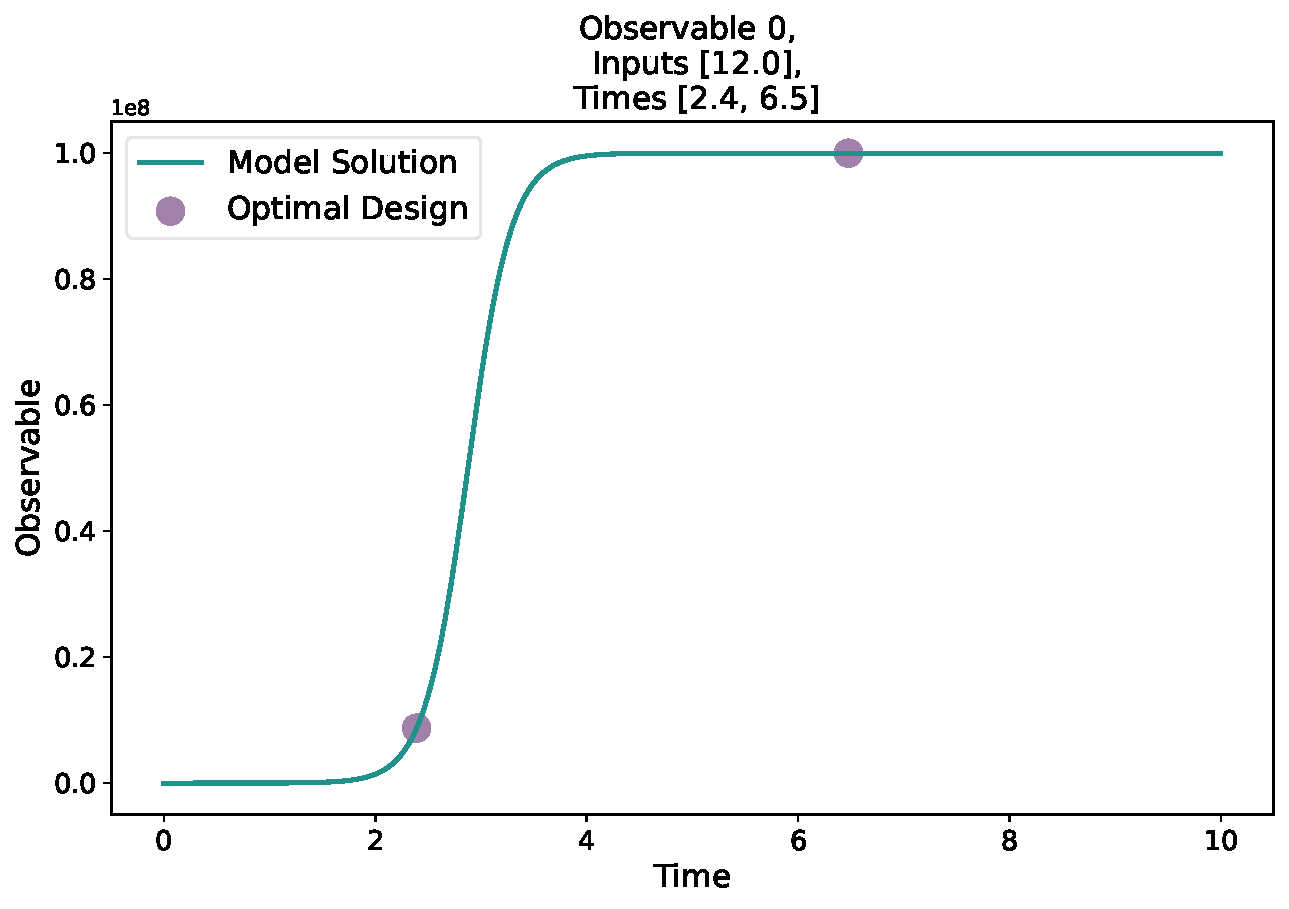
\includegraphics[scale=0.255]{Figures/Observable_Results_baranyi_roberts_ode_fisher_determinant_rel_sensit_cont_2times_2temps_000_x_00.pdf}
    \end{subfigure}  
    \begin{subfigure}{.5\textwidth}
        \centering
        \subcaption{{\footnotesize Experiment 2: $T = 12^\circ$C, $t=43\text{h}, 100$h}}
        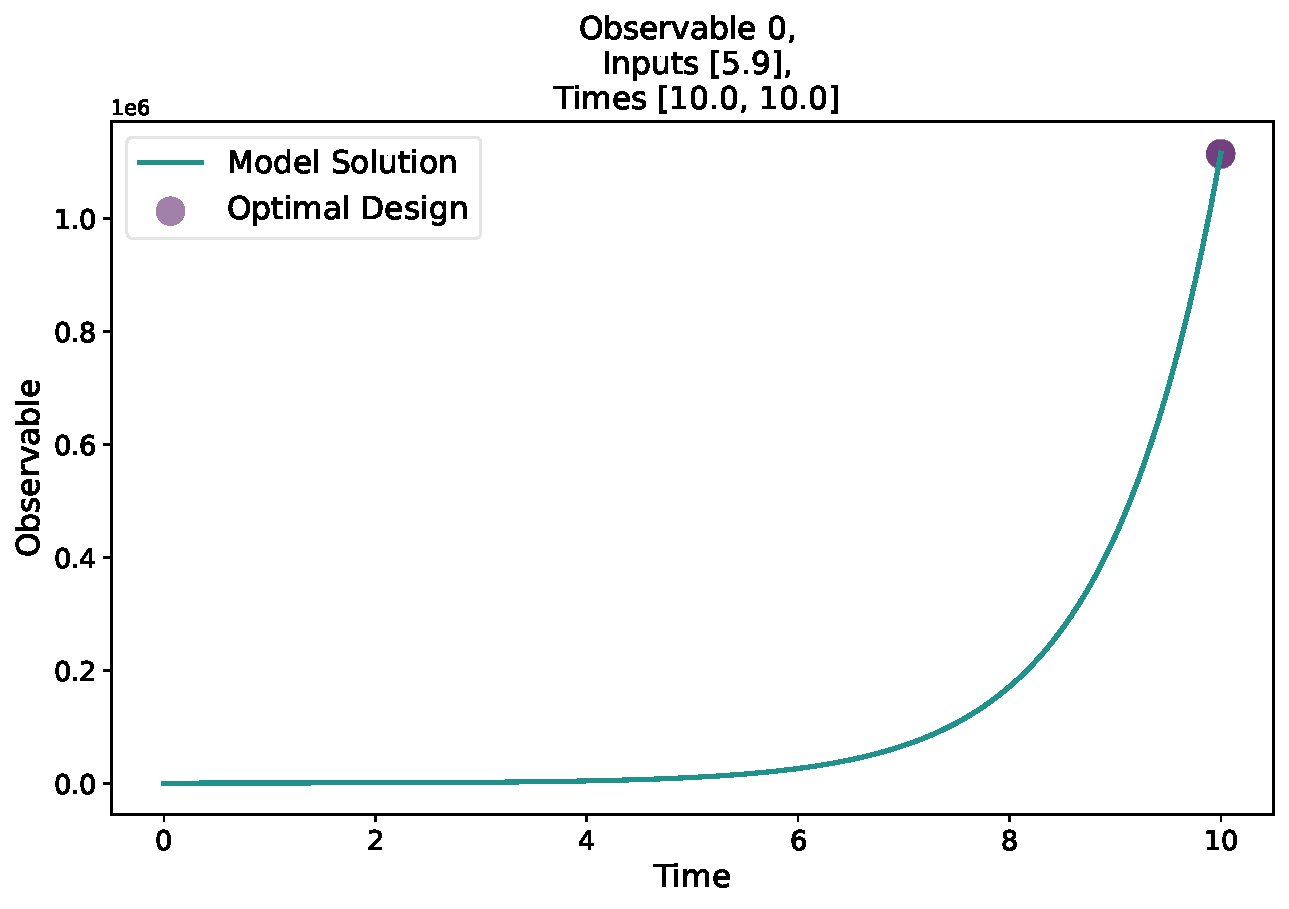
\includegraphics[scale=0.255]{Figures/Observable_Results_baranyi_roberts_ode_fisher_determinant_rel_sensit_cont_2times_2temps_001_x_00.pdf}
    \end{subfigure}
    \caption{{\footnotesize The example of the output of the Experimental Design optimization procedure for the Baranyi and Roberts model.
    The line plot presents the model solution for the observable, and the circles determine the suggested by Experimental Design time points.
    The Optimal Design is proposed for one observable which is the total bacterial count of the species $x_1$ and consists of two time series where samples are stored at temperatures (a) $T_1 = 3.5^\circ$C and (b) $T_2 = 12^\circ$C.
    The corresponding measurement times are (a)~$t_{11}=100$h and (b)~$t_{21}=43$h, $t_{22}=100$h.}}
    \label{fig:baranyi_roberts_observable}
\end{figure}
\begin{figure}[H]
    \centering
    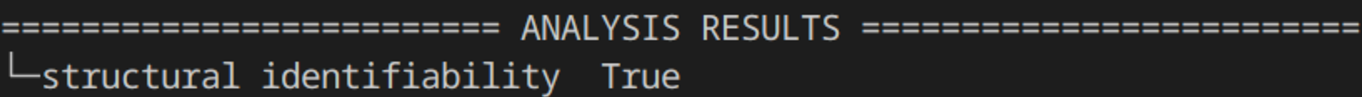
\includegraphics[scale=0.5]{Figures/ident_check_output.pdf}
    \caption{{\footnotesize The result of the identifiability check for the Experimental Design provided in Figure~\ref{fig:baranyi_roberts_observable}.
    The output shows that the Experimental Design gives structurally identifiable result and allows to estimate parameters of the system.}}
    \label{fig:identif_check}
\end{figure}
For the system described above the minimal requirements for passing the identifiability test (see Figure~\ref{fig:identif_check}) is using a setup with at least two temperatures and two measurement times per temperature.
The choice of minimal number of measurement times can also be justified when looking at Figure~\ref{fig:det_vs_ntimes}.
Here we see that one measurement time is not enough as the determinant is numerically very close to zero indicating a non-identifiability of this systems configuration.
%
\begin{figure}[H]
    \begin{subfigure}{.5\textwidth}
      \centering
      \subcaption{{\footnotesize $T_1=3.5^\circ$C, parameter $x_\text{max}$}}
      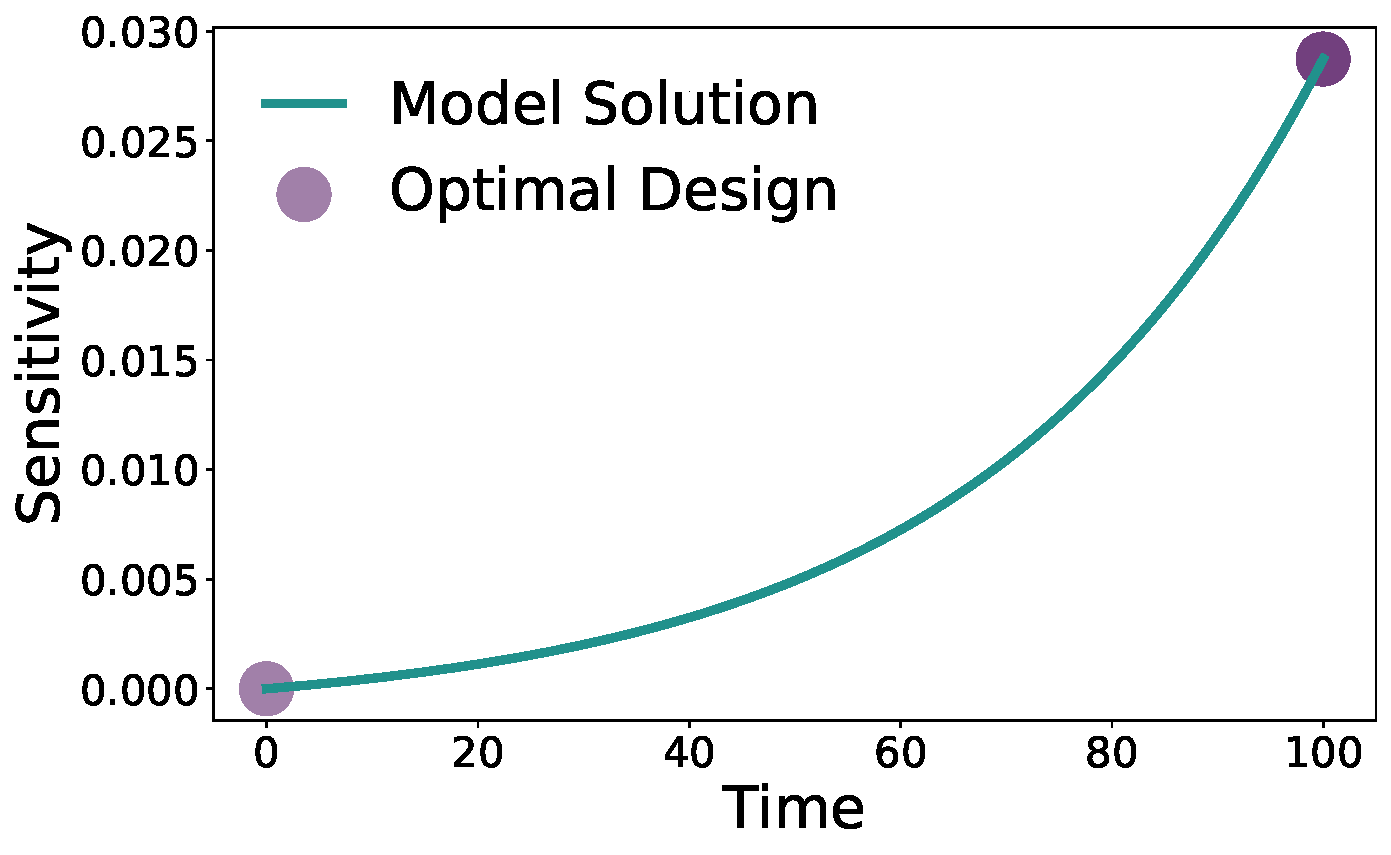
\includegraphics[scale=0.255]{Figures/Sensitivity_Results_baranyi_roberts_ode_fisher_determinant_rel_sensit_cont_2times_2temps_000_x_00_p_00.pdf}
    \end{subfigure}
    \begin{subfigure}{.5\textwidth}
        \centering
        \subcaption{{\footnotesize $T_2=12^\circ$C, parameter $x_\text{max}$}}
        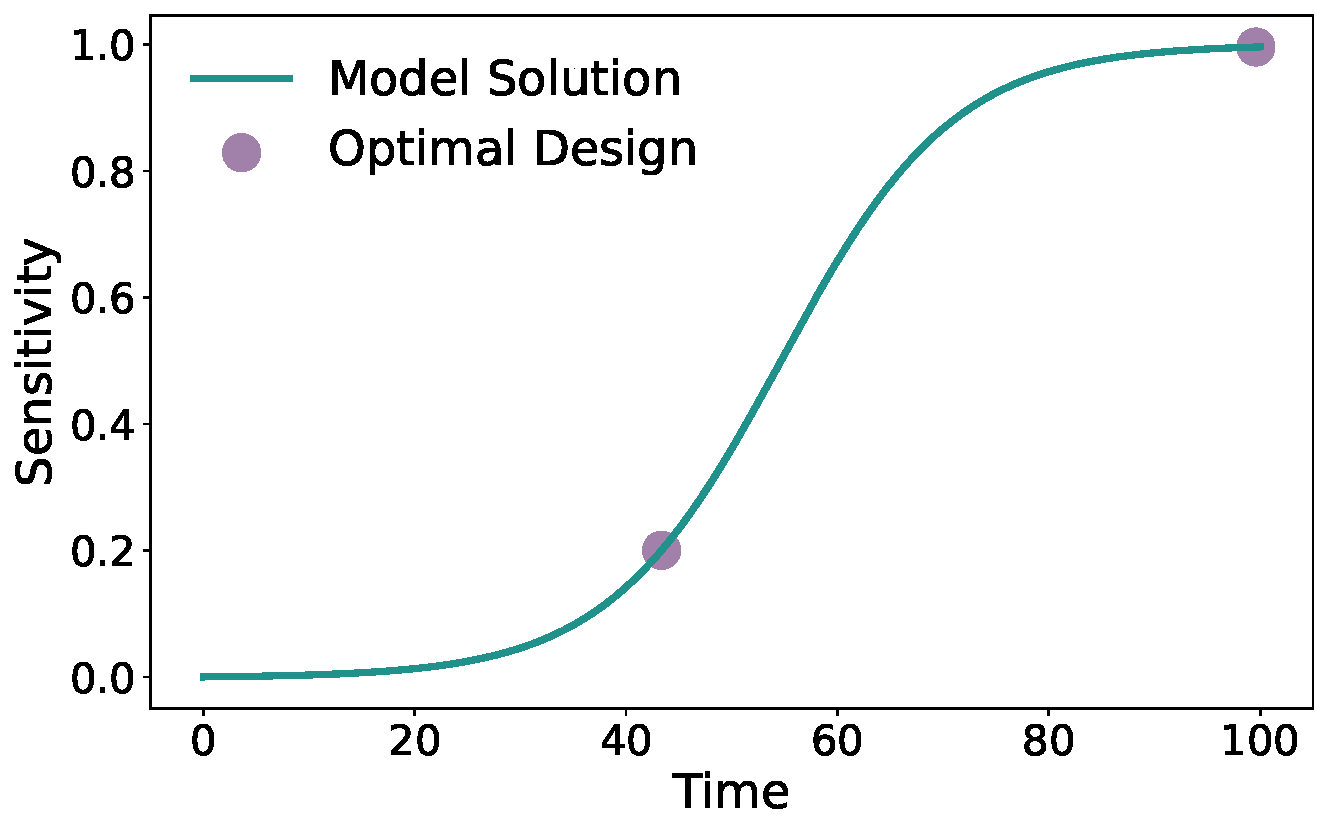
\includegraphics[scale=0.255]{Figures/Sensitivity_Results_baranyi_roberts_ode_fisher_determinant_rel_sensit_cont_2times_2temps_001_x_00_p_00.pdf}
    \end{subfigure}
    \begin{subfigure}{.5\textwidth}
      \centering
      \subcaption{{\footnotesize $T_1=3.5^\circ$C, parameter $b$}}
      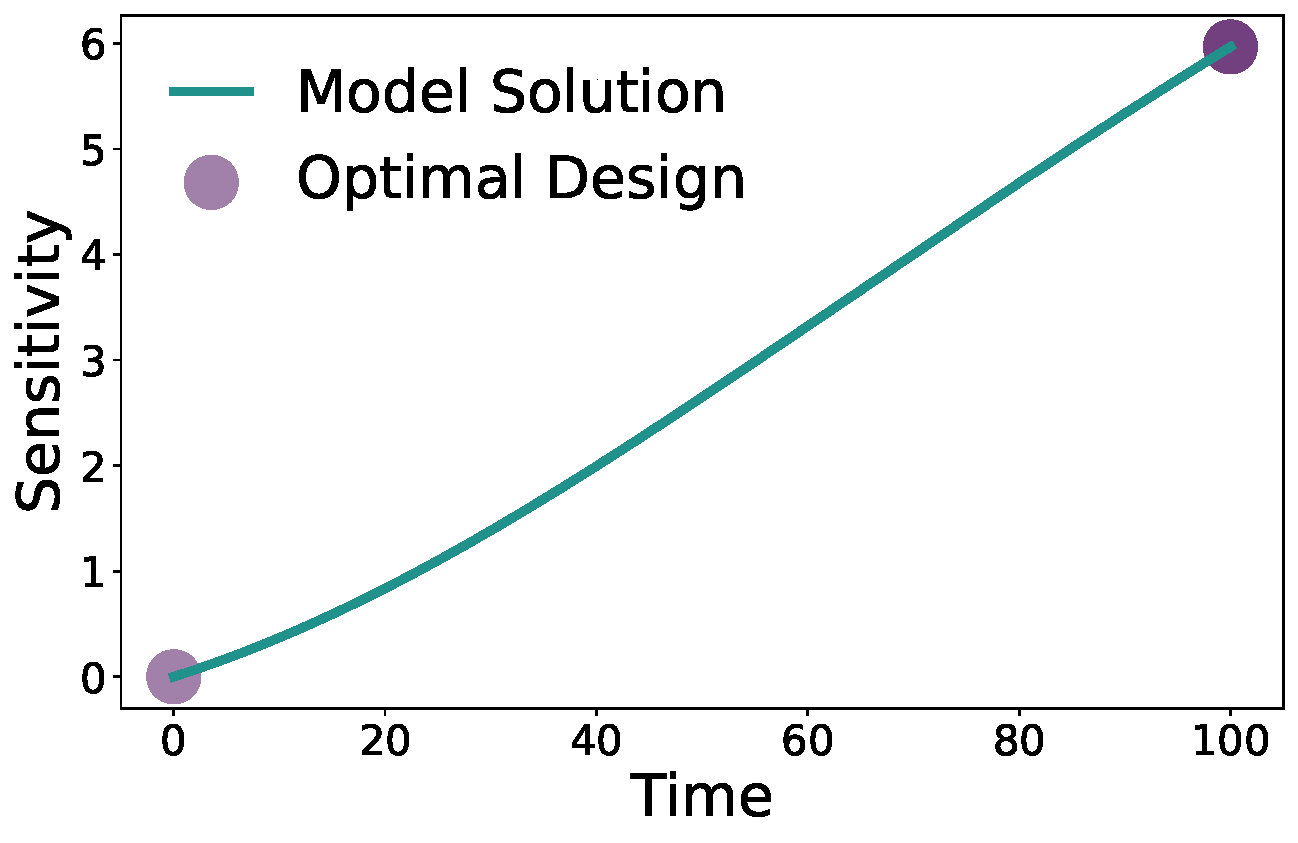
\includegraphics[scale=0.255]{Figures/Sensitivity_Results_baranyi_roberts_ode_fisher_determinant_rel_sensit_cont_2times_2temps_000_x_00_p_01.pdf}
    \end{subfigure}
    \begin{subfigure}{.5\textwidth}
        \centering
        \subcaption{{\footnotesize $T_2=12^\circ$C, parameter $b$}}
        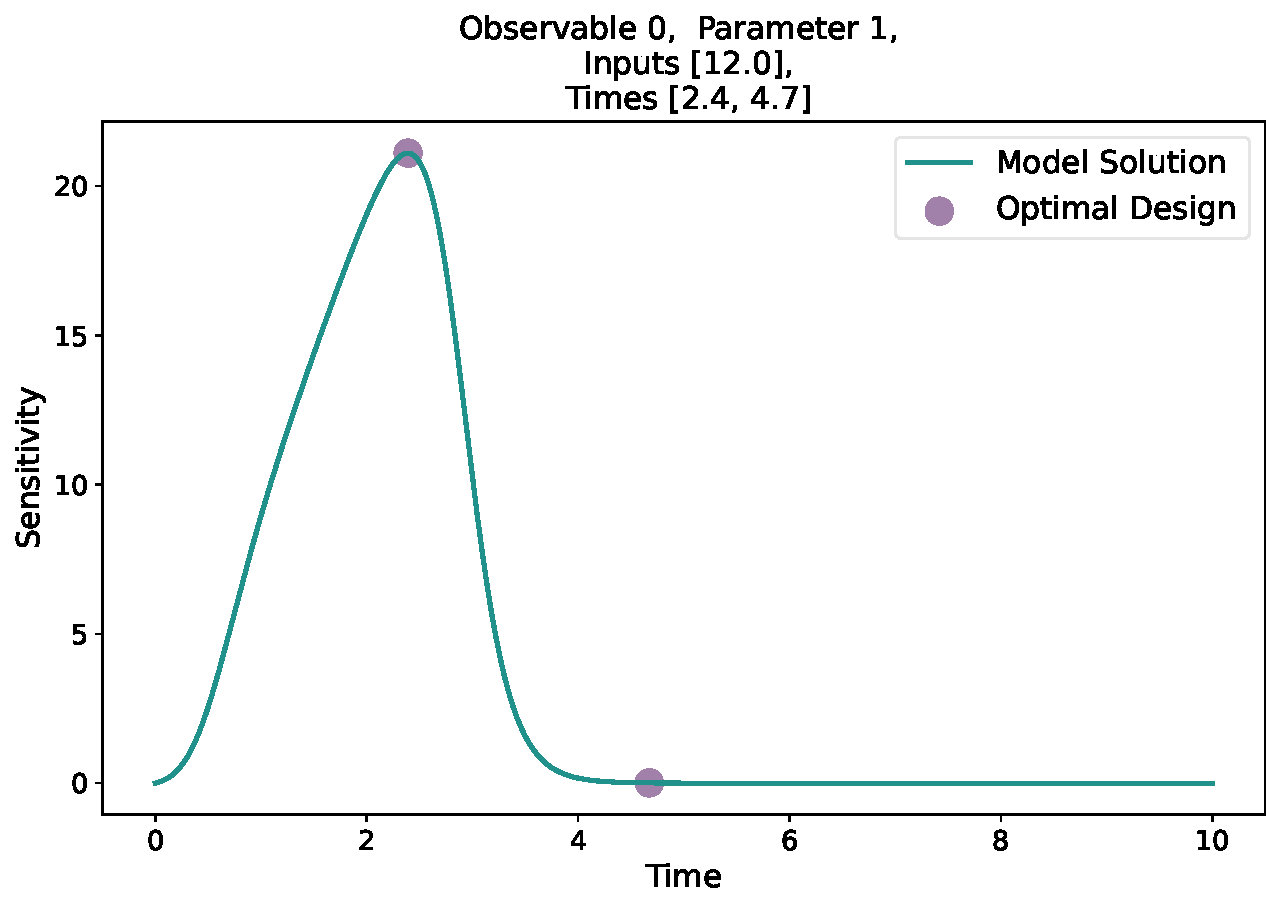
\includegraphics[scale=0.255]{Figures/Sensitivity_Results_baranyi_roberts_ode_fisher_determinant_rel_sensit_cont_2times_2temps_001_x_00_p_01.pdf}
    \end{subfigure}
    \begin{subfigure}{.5\textwidth}
        \centering
        \subcaption{{\footnotesize $T_1=3.5^\circ$C, parameter $T_\text{min}$}}
        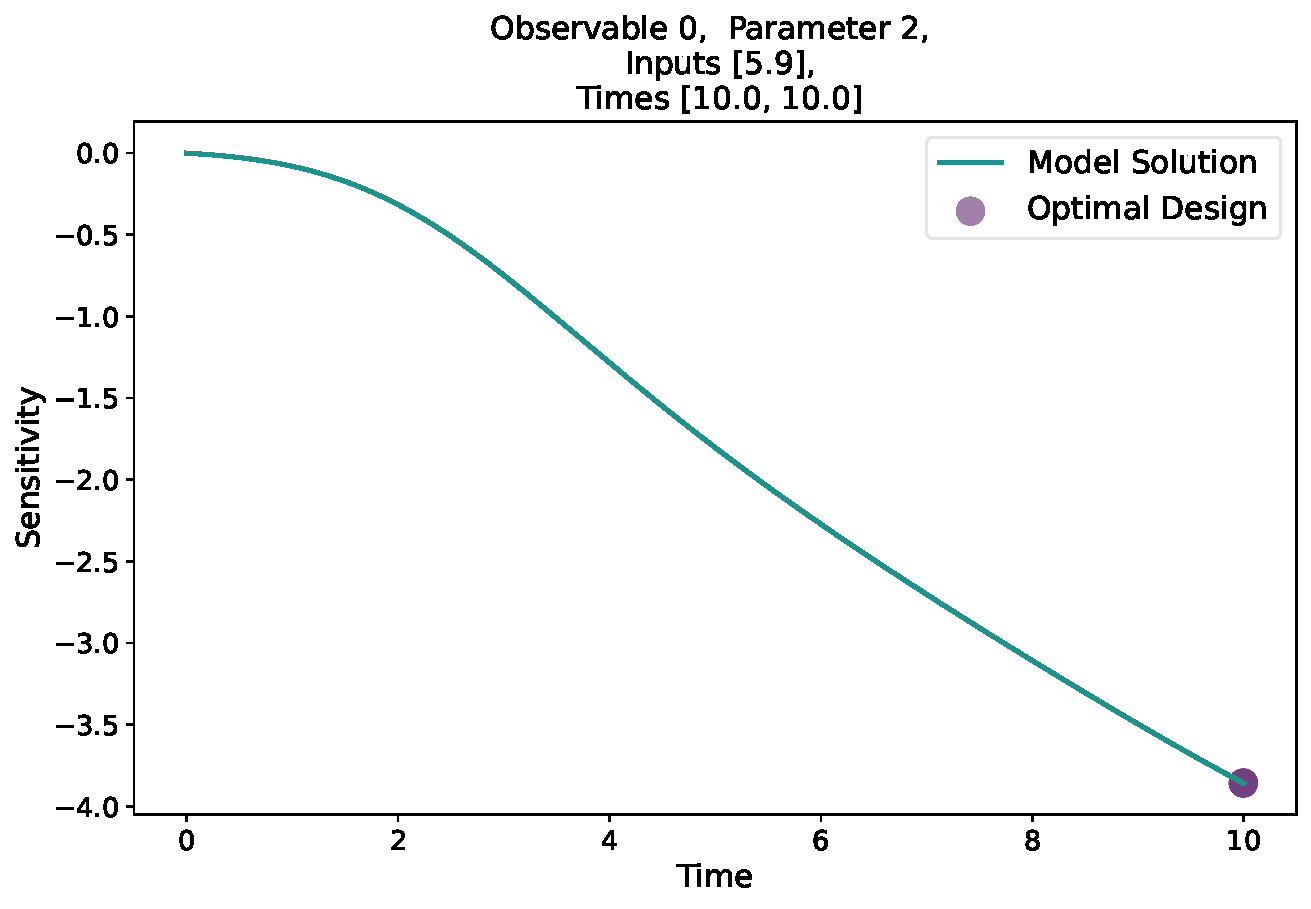
\includegraphics[scale=0.255]{Figures/Sensitivity_Results_baranyi_roberts_ode_fisher_determinant_rel_sensit_cont_2times_2temps_000_x_00_p_02.pdf}
    \end{subfigure}
    \begin{subfigure}{.5\textwidth}
          \centering
          \subcaption{{\footnotesize $T_2=12^\circ$C, parameter $T_\text{min}$}}
          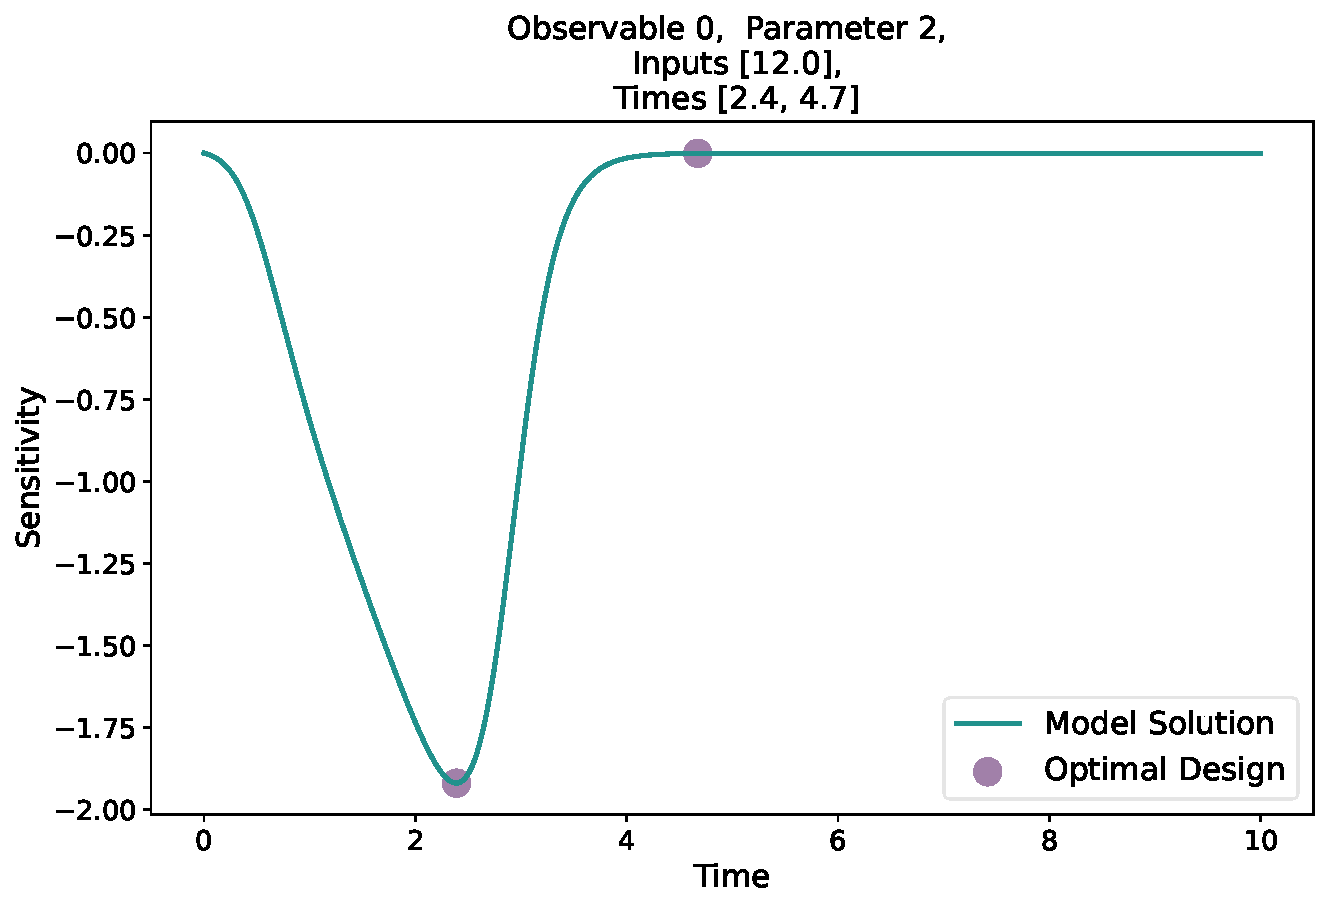
\includegraphics[scale=0.255]{Figures/Sensitivity_Results_baranyi_roberts_ode_fisher_determinant_rel_sensit_cont_2times_2temps_001_x_00_p_02.pdf}
        \end{subfigure}
    \caption{{\footnotesize The example of the sensitivities of the total bacterial count calculated for the Experimental Design optimization procedure for the Baranyi and Roberts model.
    The line plot presents the model solution for the observable, and the circles determine the suggested by Experimental Design time points.
    In (a), (c), (e) the sensitivity curves for the experimental series at storage temperature $T_1=3.5^\circ$C are shown for parameters $x_\text{max}$, $b$, $T_\text{min}$, respectively.
    As well as, (b), (d), (f) subfigures present the sensitivities for the $T_2=12^\circ$C experiment for parameters $x_\text{max}$, $b$, $T_\text{min}$, respectively.}}
    \label{fig:baranyi_roberts_sensitivities}
\end{figure}
Figure~\ref{fig:baranyi_roberts_sensitivities} shows that each of the chosen optimal time points corresponds to the maximum of at least one local sensitivity curve.
This maximizes the determinant of the Fisher Information matrix.
%
%
%
\begin{figure}[H]
    \centering
    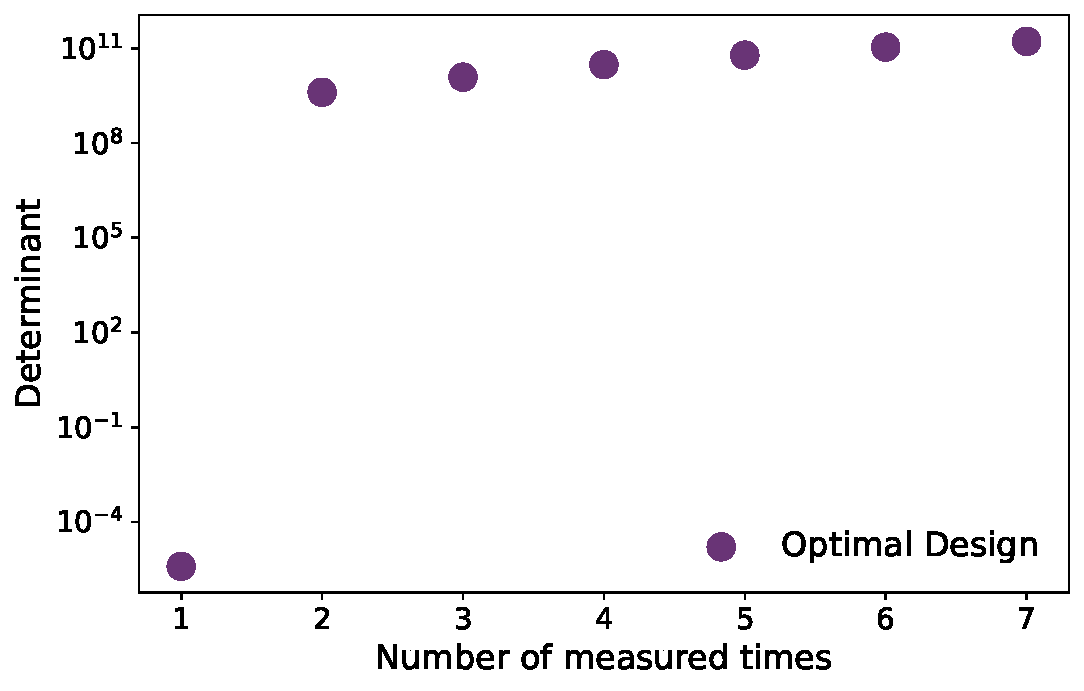
\includegraphics[scale=0.4]{Figures/det_vs_ntimes.pdf}
    \caption{{\footnotesize The determinant of the \ac{fim} as a function of the number of measurement times for the Experimental Design consisted of two measured temperatures.}}
    \label{fig:det_vs_ntimes}
\end{figure}
%
%
%
\subsection*{Two-Species Resource Competition}
As a second example we discuss a slightly more complicated system and extend the previous example of bacterial growth to a system where two species are present.
The species interact by competitive inhibition because they depend on a common nutrient resource.
Analogously to the previous example, we denote the concentration of the two different species as $x_1$ and $y_1$, respectively.
The system can be described by the following set of \acp{ode}:
\begin{equation}
    \begin{cases}
        \dot x_1 = \alpha_x R x_1 \\
        \dot y_1 = \alpha_y R y_1 \\
        \dot R = -\frac{R}{n_\text{max}}(\alpha_x x_1+\alpha_y y_1)
    \end{cases}
    \label{eq:Lotka_Volterra_2species_1}
\end{equation}
where $\alpha_x, \alpha_y$ are the time and temperature dependent growth rates for population $x_1$, $y_1$, and $R$ represents the nutrient pool concentration, respectively.
Using the conservation quantity $x_1 + y_1 + n_\text{max}R = n_\text{max}$ this system can be reduced to:
\begin{equation}
    \begin{cases}
        \dot x_1 = \alpha_x x_1\left(1-\frac{x_1+y_1}{n_\text{max}}\right) \\
        \dot y_1 = \alpha_y y_1\left(1-\frac{x_1+y_1}{n_\text{max}}\right).
    \end{cases}
    \label{eq:Lotka_Volterra_2species_2}
\end{equation}
Based on the one species case for the growth rates we use \cite{baranyiDynamicApproach1994,ratkowsky_relationship_1982}
\begin{eqnarray}
    \alpha_x (t, T) = b_x^2 (T - T_{\text{min}, x})^2 \frac{x_2(t)}{x_2(t) + 1}\\
    \alpha_y (t, T) = b_y^2 (T - T_{\text{min}, y})^2 \frac{y_2(t)}{y_2(t) + 1}
    \label{eq:growth_rate_2species}
\end{eqnarray}
Combining equations (\ref{eq:Lotka_Volterra_2species_2}, \ref{eq:growth_rate_2species}), we get the system of four differential equations:
\begin{equation}
    \begin{cases}
        \dot x_1 = b_x^2 (T - T_{\text{min}, x})^2 \frac{x_2}{x_2 + 1} x_1 (1 - \frac{x_1 + y_1}{n_\text{max}})\\
        \dot x_2 = b_x^2 (T - T_{\text{min}, x})^2 x_2 \\
        \dot y_1 = b_y^2 (T - T_{\text{min}, y})^2 \frac{y_2}{y_2 + 1} y_1 (1 - \frac{x_1 + y_1}{n_\text{max}})\\
        \dot y_2 = b_y^2 (T - T_{\text{min}, y})^2 y_2 \\
    \end{cases}
    \label{eq:model_2species_resource}
\end{equation}
where $x_2, y_2$ are the concentration of the quantities determining the critical substance (nutrient) needed for growth of the species $x_1$ and $y_1$, respectively.
The values of the parameter vector $\mbp = (n_\text{max}, b_x, T_{\text{min}, x}, b_y, T_{\text{min}, y})$ and the vector of the initial values $\mbx(t_0)=(x_1(t_0), x_2(t_0), y_1(t_0), y_2(t_0))$ are presented in Table~\ref{tab:2species_vals}.
\begin{table}[H]
    \centering
    \begin{tabular}{ccc}
    \specialrule{.1em}{.01em}{.05em}
    \textbf{Variable}\hspace{3mm} & \textbf{Value}\hspace{3mm} & \textbf{Units}\\
    \toprule
    $n_\text{max}$                & $2 \cdot 10^4$             & cfu/g                                     \\
    $b_x$                         & 0.03                       & ${^\circ \text{C}}^{-1}{\text{h}^{-1/2}}$ \\
    $T_{\text{min}, x}$           & -8.0                       & ${^\circ \text{C}}$                       \\
    $b_y$                         & 0.04                       & ${^\circ \text{C}}^{-1}{\text{h}^{-1/2}}$ \\
    $T_{\text{min}, y}$           & -5.5                       & ${^\circ \text{C}}$                       \\
    \midrule
    $x_1(t_0)$                      & 50.0                       & cfu/g                                     \\
    $x_2(t_0)$                      & 1.0                        &      1                                     \\
    $y_1(t_0)$                      & 20.0                       & cfu/g                                     \\
    $y_2(t_0)$                      & 1.0                        &      1                                     \\
    \bottomrule
    \end{tabular}
    \caption{{\footnotesize The list of the parameter and \ac{ode}'s initial values of the system that fully define the system~(\ref{eq:model_2species_resource}).}}
    \label{tab:2species_vals}
\end{table}
In comparison to the previous example, we now choose the count of the two bacteria species $x_1,y_1$ as observables.
Meanwhile other optimization arguments were taken the same as in the previous example ie. we optimize measurement times and temperatures.
The new \ac{oed} is shown in Figure \ref{fig:baranyi_roberts_2species_observable}.
\begin{figure}[H]
    \begin{subfigure}{.5\textwidth}
        \centering
        \subcaption{{\footnotesize Species 1, $T = 12^\circ$C, $t=12 \text{h}, 38$h}}
        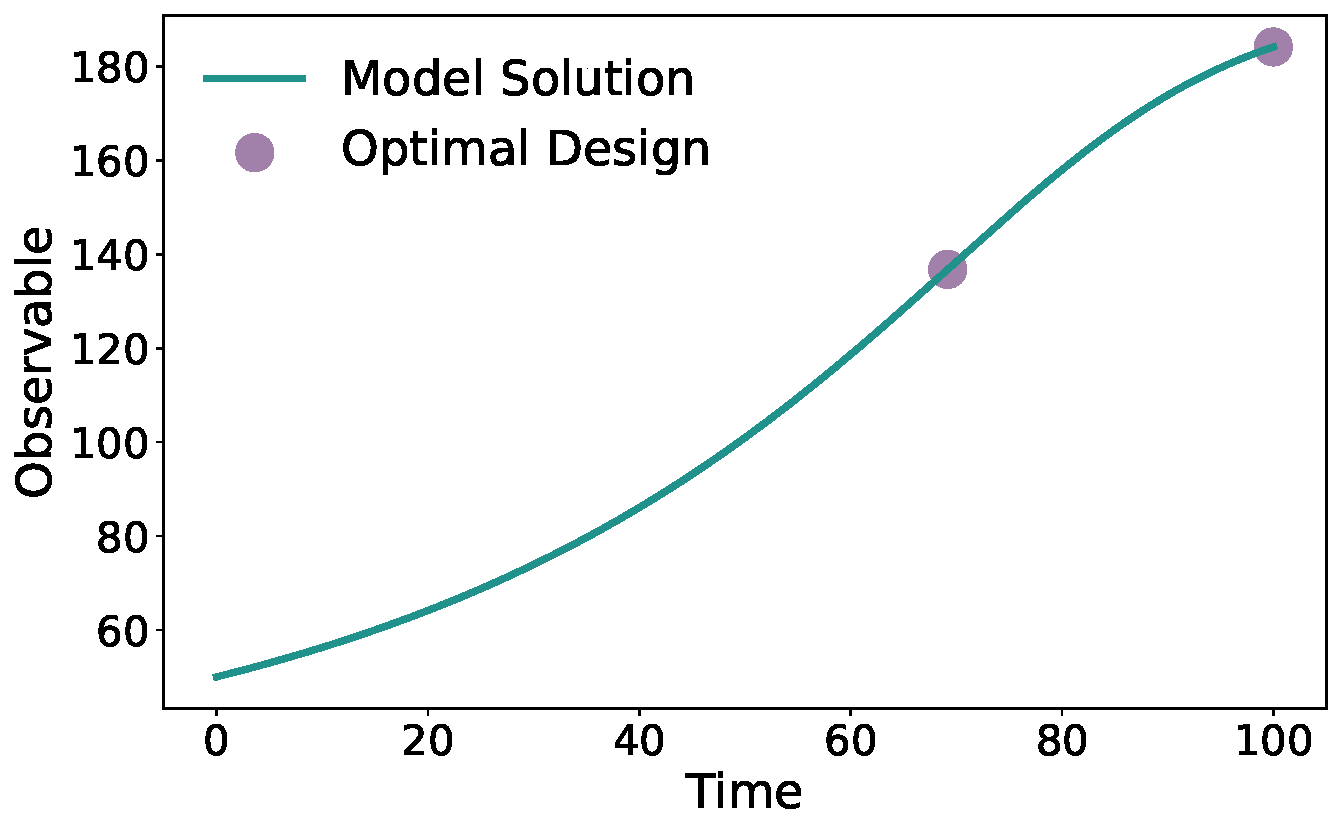
\includegraphics[scale=0.255]{Figures/Observable_Results_baranyi_roberts_ode_fisher_determinant_2species_rel_sensit_cont_2times_2temps_000_x_00.pdf}
      \end{subfigure} 
    \begin{subfigure}{.5\textwidth}
        \centering
        \subcaption{{\footnotesize Species 1, $T = 2^\circ$C, $t=58 \text{h}, 90$h}}
        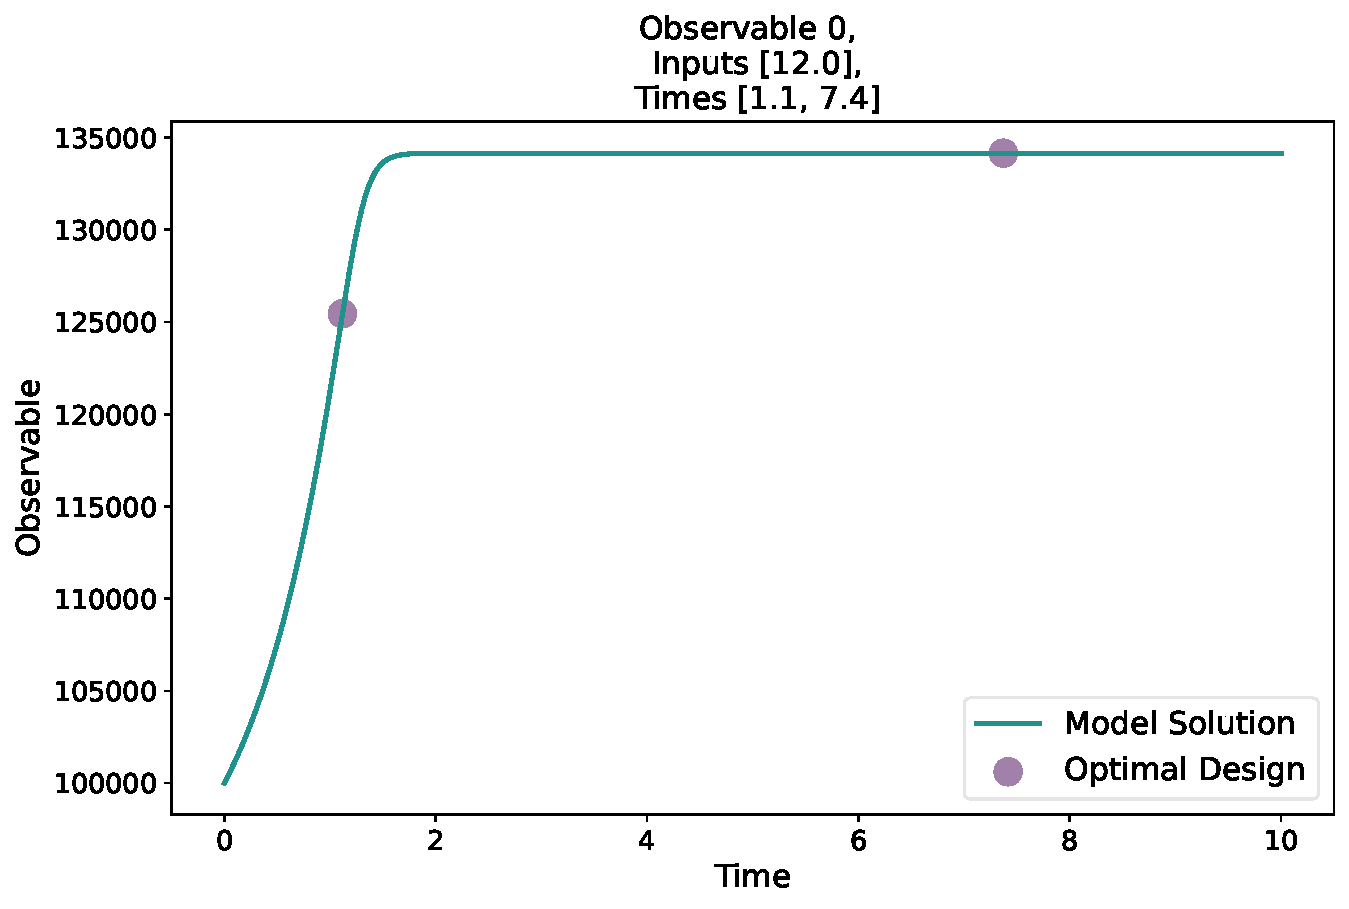
\includegraphics[scale=0.255]{Figures/Observable_Results_baranyi_roberts_ode_fisher_determinant_2species_rel_sensit_cont_2times_2temps_001_x_00.pdf}
    \end{subfigure}
      \begin{subfigure}{.5\textwidth}
        \centering
        \subcaption{{\footnotesize Species 2, $T = 12^\circ$C, $t=12 \text{h}, 38$h}}
        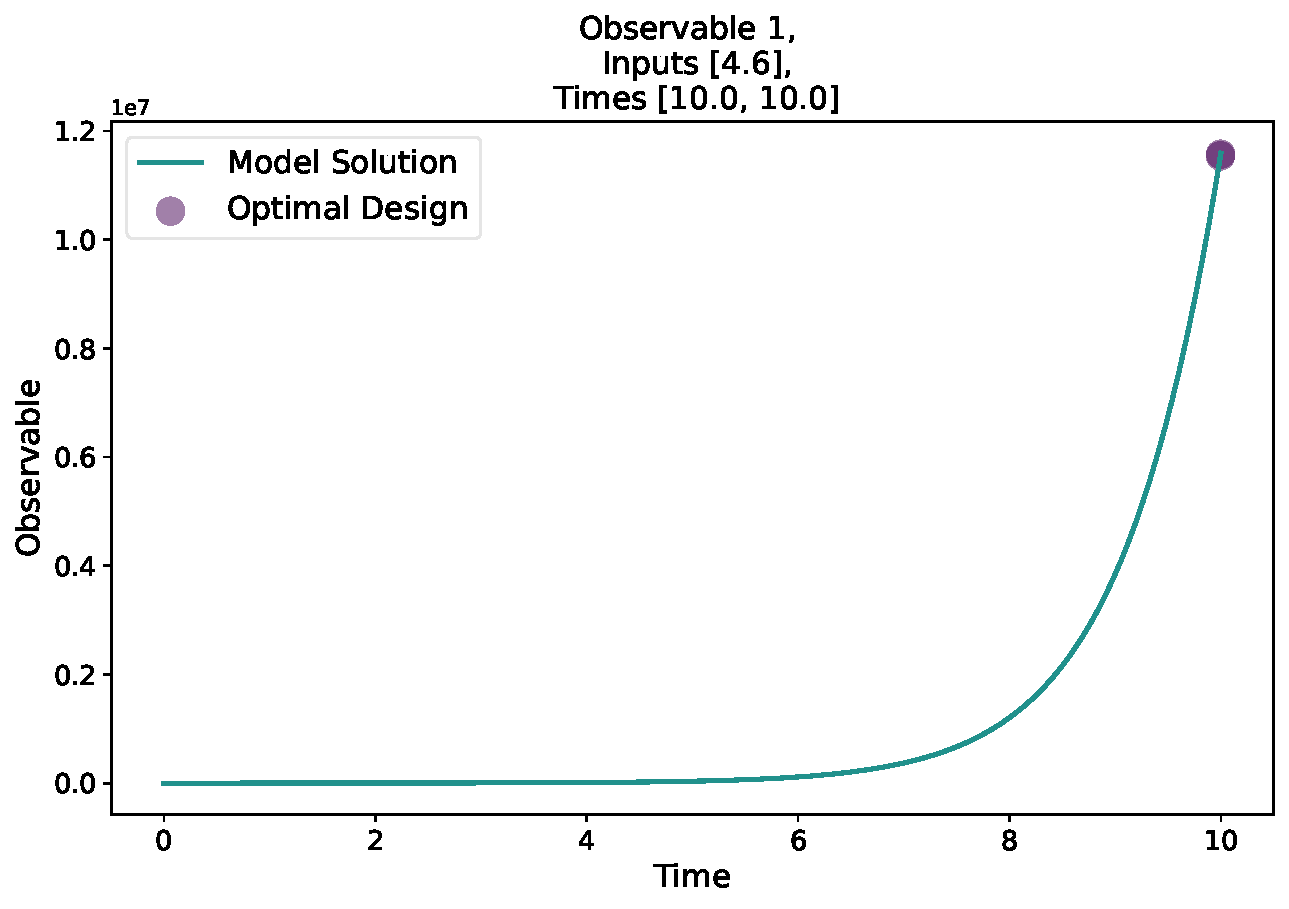
\includegraphics[scale=0.255]{Figures/Observable_Results_baranyi_roberts_ode_fisher_determinant_2species_rel_sensit_cont_2times_2temps_000_x_01.pdf}
    \end{subfigure}
    %\end{figure}%
    %\begin{figure}[H]\ContinuedFloat      
    \begin{subfigure}{.5\textwidth}
        \centering
        \subcaption{{\footnotesize Species 2, $T = 2^\circ$C, $t=58 \text{h}, 90$h}}
        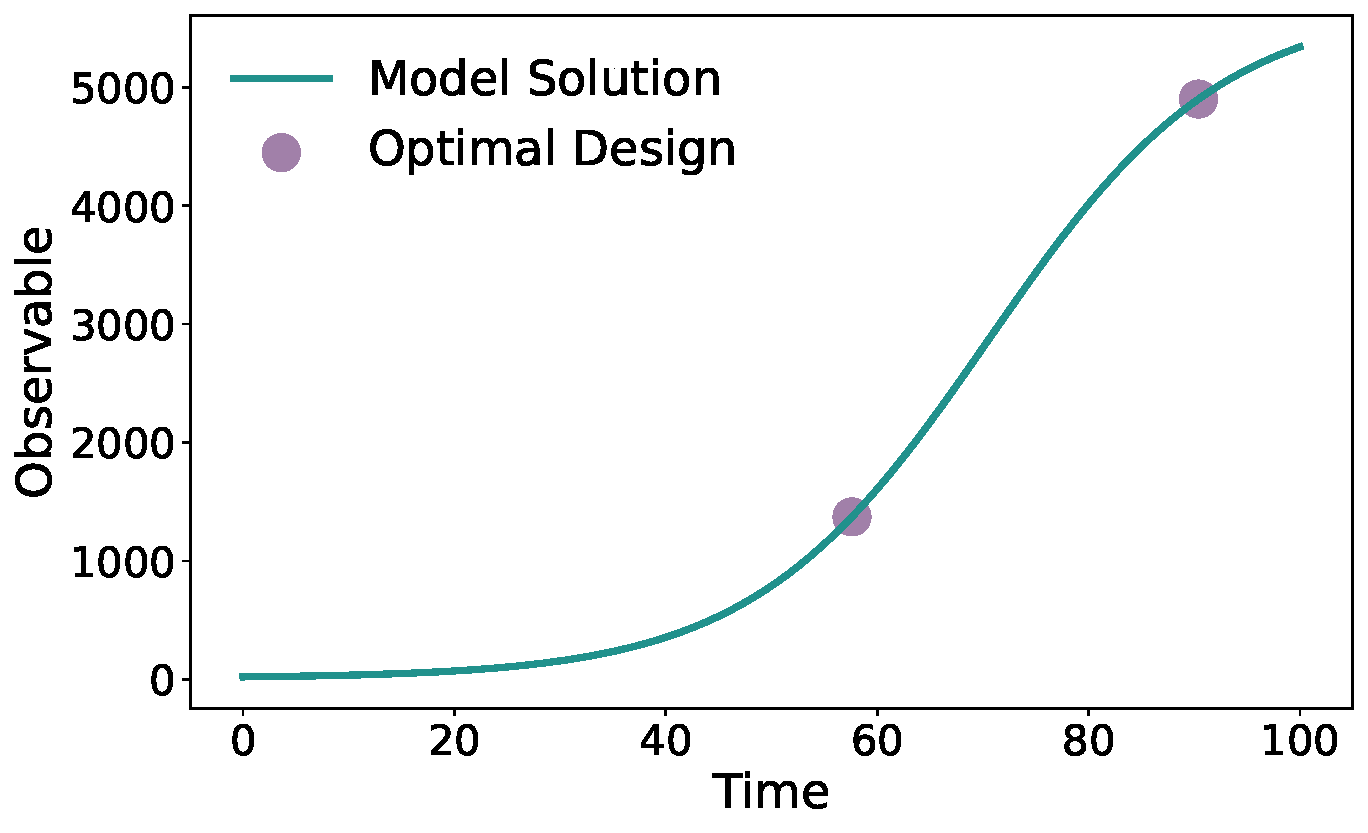
\includegraphics[scale=0.255]{Figures/Observable_Results_baranyi_roberts_ode_fisher_determinant_2species_rel_sensit_cont_2times_2temps_001_x_01.pdf}
    \end{subfigure} 
    \caption{{\footnotesize
    The Optimal Experimental Design for the Baranyi and Roberts model with two different species~(\ref{eq:model_2species_resource}) is proposed for two observables: the bacterial count of the first species $x_1$ and of the second species $x_2$.
    (a), (c) show the first experimental series held at the temperature $T_1=12^\circ$C and with measurement times $t_{11}=12$h, $t_{12}=38$h for observables $x_1$ and $x_2$, respectively.
    (b), (d) show the second experimental series held at the temperature $T_2=2^\circ$C and with measurement times $t_{21}=58$h, $t_{22}=90$h for observables $x_1$ and $x_2$, respectively.
    The line plot presents the model solution for the observable, and the circles determine the suggested by Experimental Design time points.}}
    \label{fig:baranyi_roberts_2species_observable}
\end{figure}
%
The presented design shows that the least needed number of experiments is two with temperatures of $2^\circ$C and $12^\circ$C.
In each experiment two observables that correspond to the concentrations of two bacteria types and two time points were measured.
Note that for both temperatures at least two time-points are required for identifiability.
Thus we can estimate the parameters by performing experiments according to this design.
%
%
%
\section*{Conclusion}
We introduced the concepts of Experimental Design and identifiability and their practical applications to systems described by \acp{ode}.
In addition, we implemented the numerical calculations in simple python code which we provide within our software {\it eDPM}.
Our toolbox provides a simple way to apply methods of mathematical statistics and optimization.
We demonstrated how to use these methods by applying them to the well-known Baranyi \& Roberts model for microbial growth with one and two species.
These results show us how parameters of the model can now be estimated most precisely by designing experiments around the predicted measurement conditions.
% The output of our approach identifies the most relevant measurement conditions in order to most optimally estimate the parameters of the system.
% The calculated measurement conditions can then be further used to ...
% The main result is a concise and .... approach to finding optimal measurement conditions for many cases in microbiology.
% In summary, we enable researchers to more effectively plan their experiments based on limited resources.
In summary, model-based experimental design can accelerate and simplify the planning of efficient experiments for parameter estimation in microbiology.
%
%
%
% ########################################################################
% ########################################################################
\section*{Supporting information}
%
%
%
\nolinenumbers
% ########################################################################
% ########################################################################
\bibliography{predictive-microbiology-software}

\end{document}
